% nakagawa_thesis.tex
% ーーーーーーーーーーーーーーーーーーーーーーーーーーーーーーー

\documentclass[a4paper,12pt]{article_vdlab_sotsuron}
\pagestyle{plain}

\usepackage{setspace}
\usepackage{graphicx}
\usepackage{amsmath,amssymb}
\usepackage{colortbl}
\usepackage{comment}

\begin{document}
%文字間隔を設定
\kanjiskip = .0pt plus 3pt minus 3pt
\xkanjiskip = .0pt plus 3pt minus 3pt
\small
\setstretch{1.5}

% ーーーーーーーーーーーーーーーーーーーーーーーーーーーーーーー

\begin{center}
  % 論文題目
  \jtitle{IDCS制御手法を用いたHILSシステムの検討}
  \etitle{Investigation of HILS system using IDCS}
\end{center}

%目次の表示
\tableofcontents

% ーーーーーーーーーーーーーーーーーーーーーーーーーーーーーーー

\newpage
\section{序論}
\subsection{タイヤとサスペンション}
タイヤは自動車において唯一路面と接触する要素であり,自動車の基本的な機能である「走る」「曲がる」「止まる」といった運動は,すべてタイヤと路面の接触面に発生する摩擦力によって実現している\cite{uno}.そのため,タイヤの特性を十分理解することで車両の運動特性を把握し,その運動性能を十分に発揮させることができる\cite{nasugawa}.タイヤの状態に影響を及ぼす要因として,車体とタイヤを連結するサスペンション機構が挙げられる.サスペンションは路面入力の緩衝装置であるが,安定したコーナリングを作るためにも重要である.つまり,車の挙動を安定させタイヤの性能を十分に引き出すことがサスペンションの重要な機能である.したがって,車両運動性能を把握するためには,タイヤとサスペンションを複合的に評価する必要がある.

% ーーーーーーーーーーーーーーーーーーーーーーーーーーーーーーー
% suspension
%  ーーーーーーーーーーーーーーーーーーーーーーーーーーーーーーー

\vspace{10mm}
\begin{figure}[h!]
  \begin{tabular}{cc}
    \begin{minipage}{1.0\hsize}
      \begin{center}
	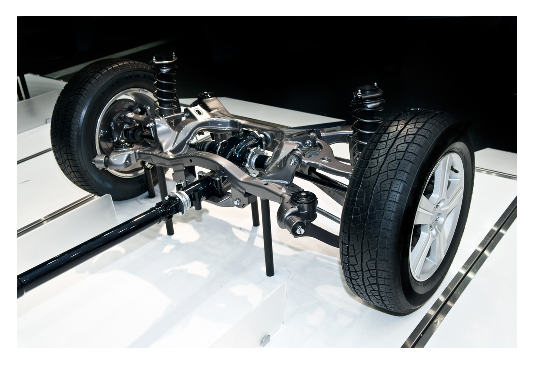
\includegraphics[scale = 1.0]{figure/pic_suspension.eps}
	\caption{Suspension System\cite{pic_sus.net}}
	\label{fig:suspension}
      \end{center}
     \end{minipage}
    \end{tabular}
\end{figure}

% ーーーーーーーーーーーーーーーーーーーーーーーーーーーーーーー
\newpage
\subsection{Hardware-in-the-Loop Simulation(HILS)システム}
車両運動性能を評価する手法として,シミュレーションや実写走行試験などが挙げられる.しかし,シミュレーションでは評価対象のモデル化誤差が生じ,実写走行試験では同一条件での試験が困難である.このような問題を解決するシステムとしてHILSシステムが用いられている\cite{exp_hils1}.HILSとはHardware-in-the-Loop Simulationの略であり,解析で得た値を目標値として実機を動かし,実機を動かすことによって得た計測値を用いてリアルタイムに解析し,実機を動かすことによって特性評価を行う手法である..従来のシミュレーションと実機試験のそれぞれの欠点を補完するようなものとなり,シミュレーション精度の向上を図りながら,試験に必要なコストを抑え,試験の自由度を確保することができる.このため,部品開発の一段階としてHILSを導入することで,制度と効率の両面において質の高い試験が可能となり,開発の大幅な効率化が期待できる\cite{exp_hils2}.

% ーーーーーーーーーーーーーーーーーーーーーーーーーーーーーーー
% hils
%  ーーーーーーーーーーーーーーーーーーーーーーーーーーーーーーー

\vspace{10mm}
\begin{figure}[h!]
  \begin{tabular}{cc}
    \begin{minipage}{1.0\hsize}
      \begin{center}
	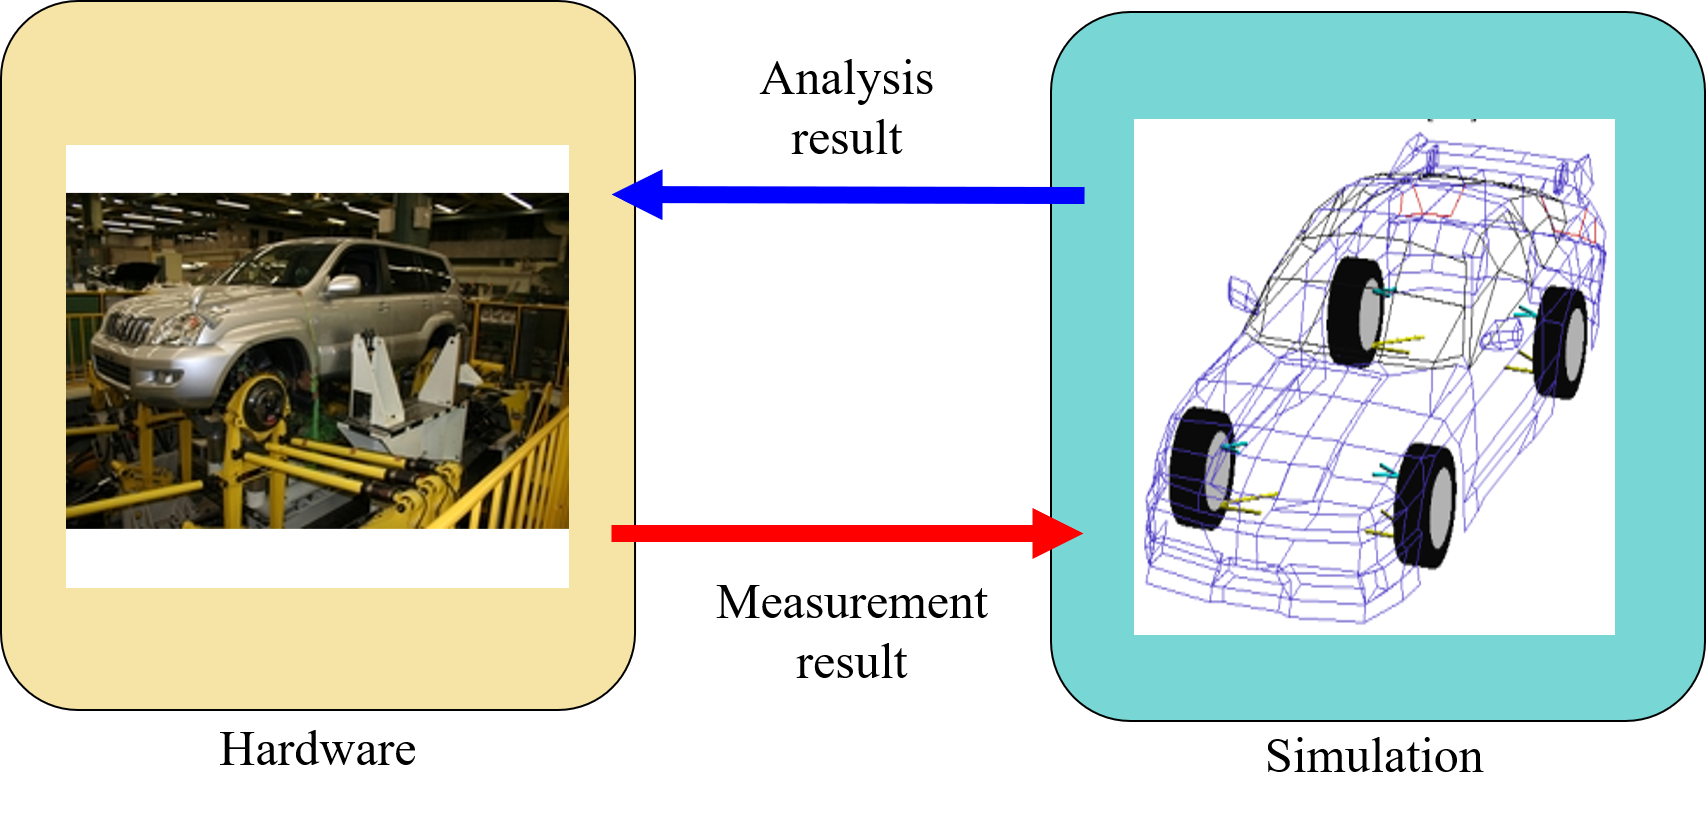
\includegraphics[scale = 0.4]{figure/hils.eps}
	\caption{HILS System\cite{toyota_hils}}
	\label{fig:HILS system}
      \end{center}
     \end{minipage}
    \end{tabular}
\end{figure}

% ーーーーーーーーーーーーーーーーーーーーーーーーーーーーーーー
\subsection{研究目的}
前述のように,HILSシステムは試験機の計測結果を用いた解析を行い,その解析結果に基づいて試験機のアクチュエータの入力を決定し特性評価を行うシステムである.HILSシステムはシミュレーション解析と実機試験の同期が必要であるため,高い制御精度が求められる.

そこで本研究では,HILSシステムの再現性の向上を目的として,Inverse Dynamics Compensation via 'Simulation of feedback control systems'(IDCS)制御手法を用いHILSシステムの制御精度の向上を行った.研究室で開発したHILS試験機を用いて,試験機の挙動と解析結果を比較することで,IDCSの有効性を検証した.また路面-車体間の相対変位を用いる制御手法による解析結果と,IDCSによる解析結果を比較し,IDCSによるHILSシステムの制御精度の優位性を検証した.

% -------------------------------------
\newpage
\section{HILSシステムの構成}
\subsection{タイヤ―サスペンションHILSシステム}
本研究で用いるタイヤ―サスペンションHILSシステムの概要を図~\ref{fig:tier-suspension HILS}~に示す.タイヤーサスペンションHILSシステムとは,計測値を用いたシミュレーション解析を行うソフトウェア部と,解析値を用いて実機試験を行うハードウェア部から構成される.本システムでは試験装置から計測されたダンパ力を用いてリアルタイムに車両運動解析を行い,ばね上ーばね下間相対変位を算出する.この解析結果に基づきアクチュエータの入力を決定し,リアルタイムに車両の上下動を再現している.

% HILSの概要図-------------------------------
\vspace{20mm}
\begin{figure}[h]
  \begin{center}
  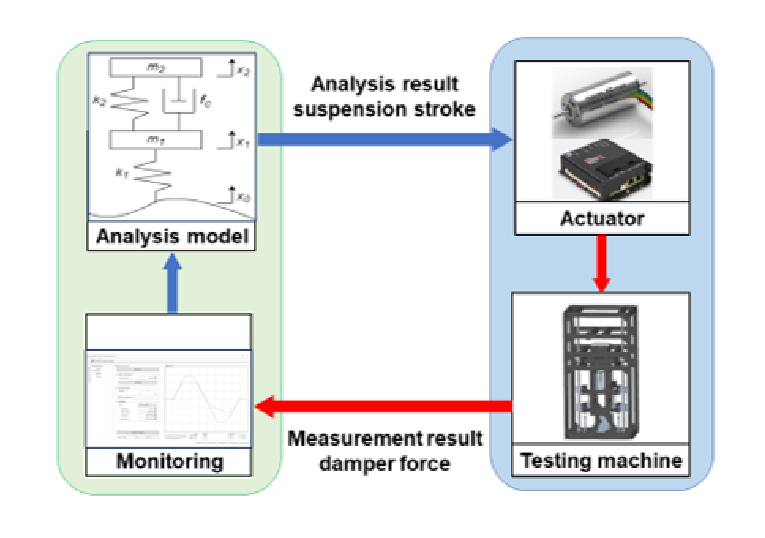
\includegraphics[height=80mm]{figure/HILS_loop.eps}
  \vspace{4mm}
   \caption{Tire-Suspension HILS System}
  \label{fig:tier-suspension HILS}
  \end{center}
\end{figure}

\newpage
\subsection{ハードウェア}
\subsubsection{HILS試験機}

本研究で用いるHILS試験機を図~\ref{fig:HILS_machine}~に示す.この装置は上下1自由度で,自動車の車体をばね上で,タイヤ-サスペンション系をばね下とばね・ダンパで表現している.また路面部にはアクチュエータを取り付けている.

ソフトウェア部で行う解析によって得たサスペンションストロークをばね上ばね下間の変位として実現している.またレーザ変位計とロードセルを用いて,サスペンションストロークとダンパ力を計測しており,ダンパ力はソフトウェア部の解析に用いられる.


% HILS_machine ---------------------------
\vspace{10mm}
\begin{figure}[h]
  \begin{center}
  \hspace{10mm}
  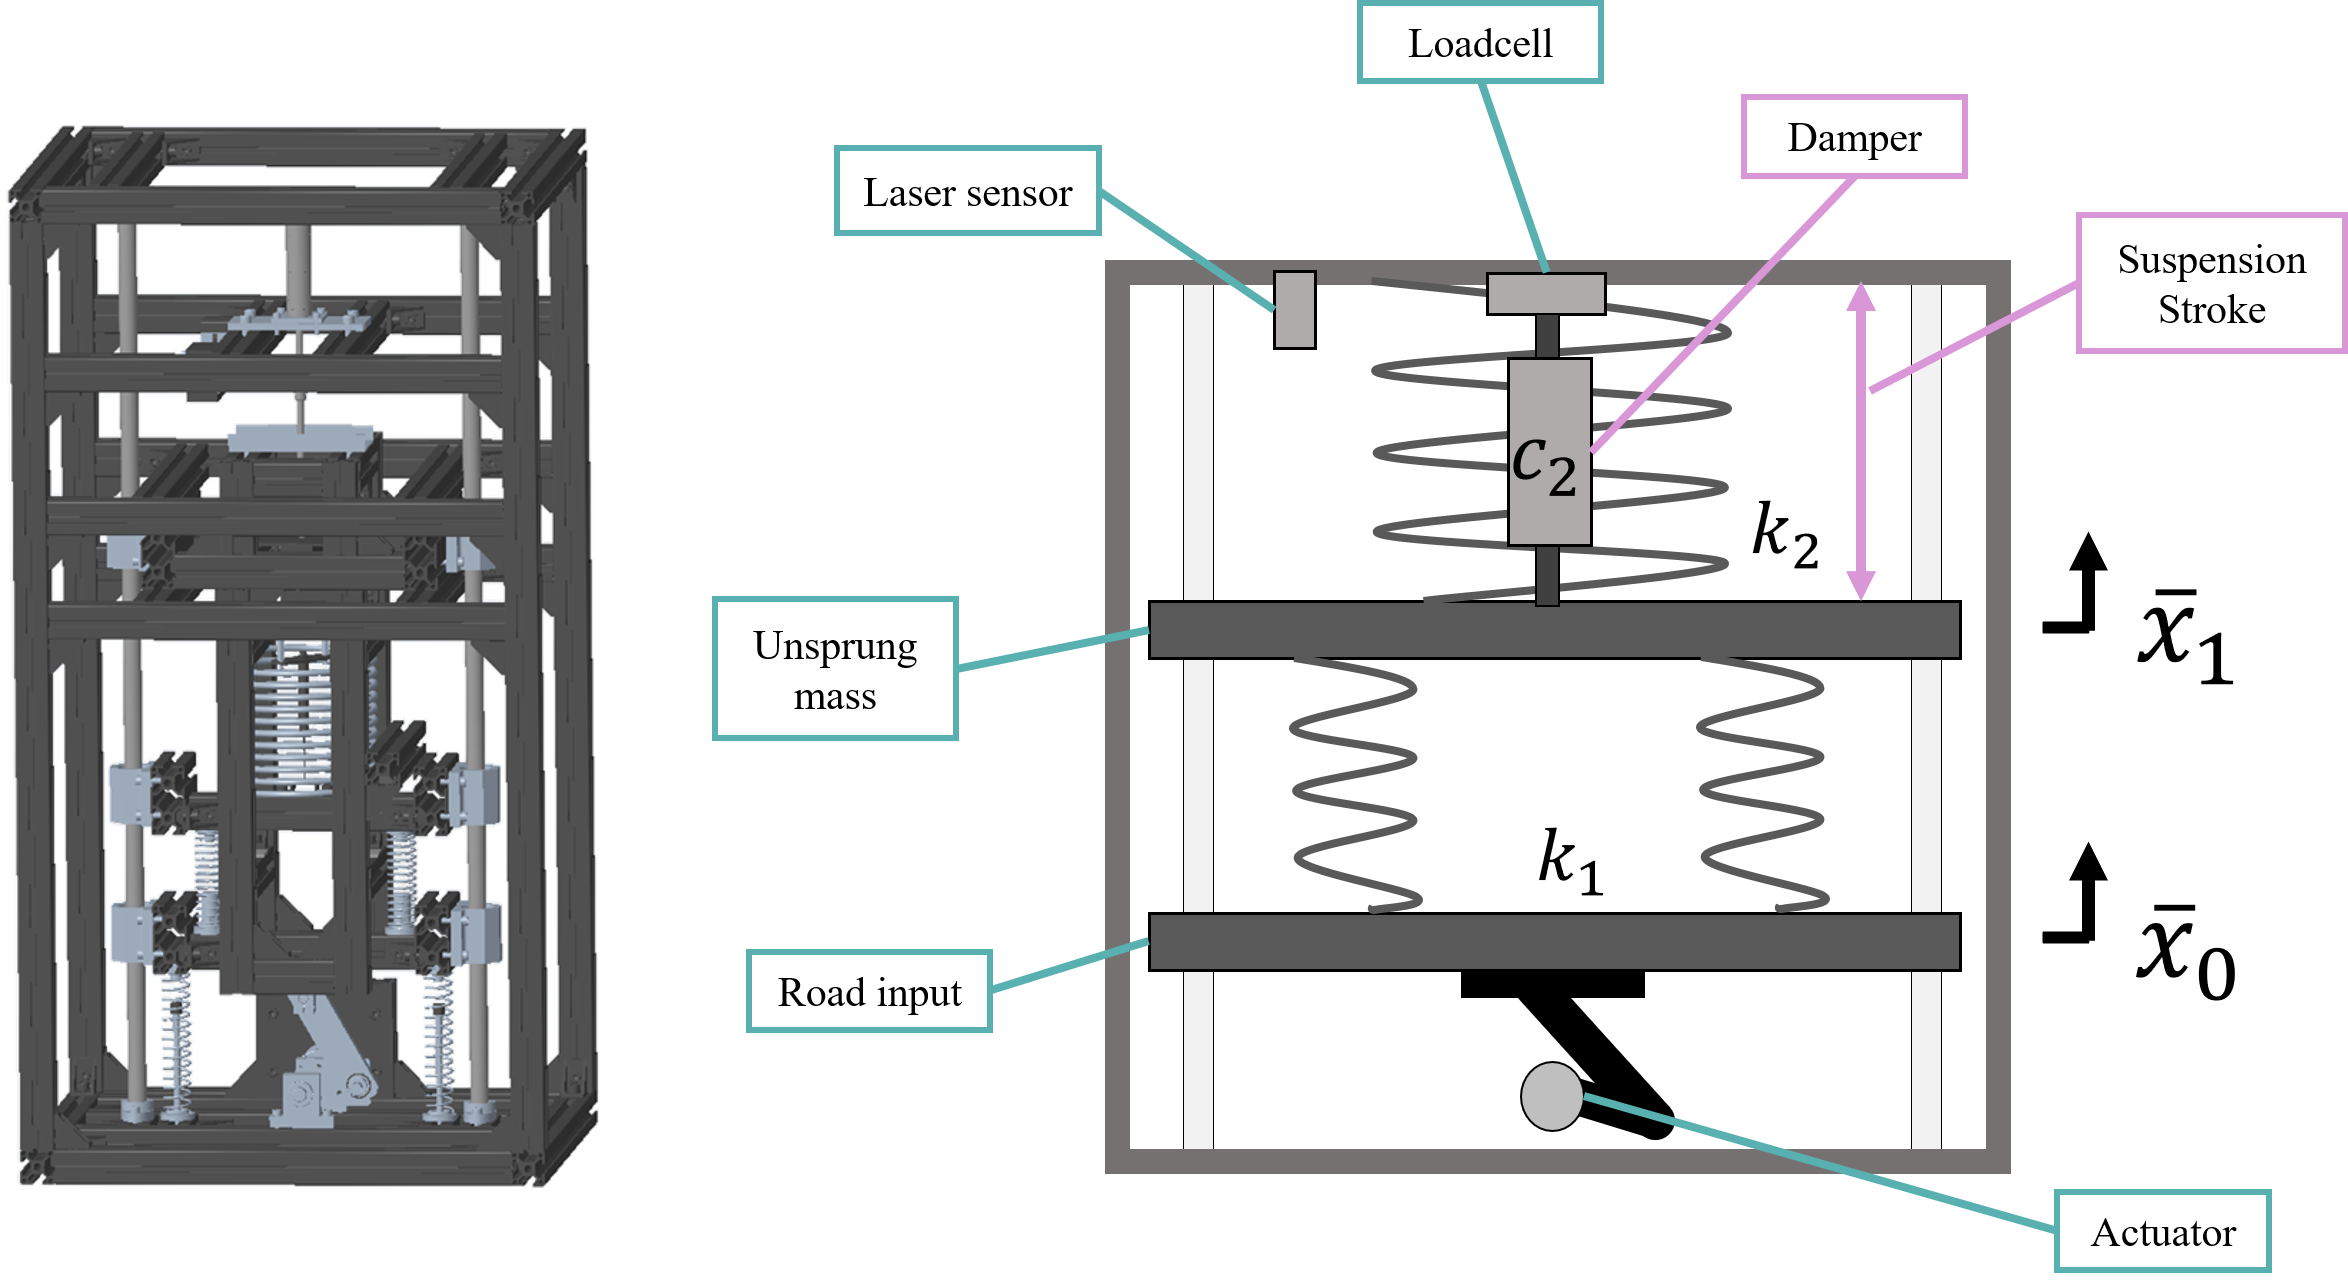
\includegraphics[height=80mm]{figure/HILS_machine.eps}
  \vspace{4mm}
   \caption{HILS Testing Machine}
  \label{fig:HILS_machine}
  \end{center}
\end{figure}

\newpage
\subsubsection{アクチュエータ}
本試験機の路面部入力を行うアクチュエータにはモータを用いる.そのモータの特性と制御ユニットとして用いるモータドライバについて説明する.

本試験機に用いるアクチュエータはmaxon$\ $japan株式会社のECモータ「EC-max$\ $40$\ $283867」である.モータの外観を図~\ref{}~に,モータスペックを表~\ref{tab:ecmax40}~に示す.モータの先端にはギアヘッドが取り付けてあり,回転方向や角度を検出する電子部品としてエンコーダが取り付けられている.このモータにはmaxon$\ $japan株式会社のブラ寝たりギアヘッド「GP42C$\ $203126」とエンコーダ「HEDL55405540$\ $115016」を取り付けた.それぞれの仕様を表~\ref{tab:Gearhead}~,表~\ref{tab:Encoder}~に示す.

% アクチュエータ性能----------------------
\vspace*{10mm}
\begin{figure}[htp]
  \begin{minipage}{0.4\textwidth}
    \begin{center}
      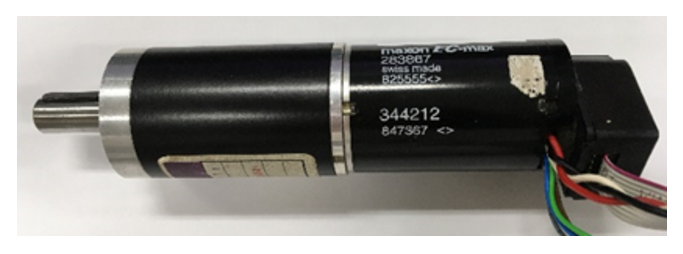
\includegraphics[height=20mm]{figure/ecmax40.eps}
      \vspace*{3mm}
      \caption{ECmax40 283867}
      \label{fig:ecmax40}
    \end{center}
  \end{minipage}
  \begin{minipage}{0.6\textwidth}
      \begin{center}
	\makeatletter
	\def\@captype{table}
	\makeatother
	\caption{Specification of EC Servomotor(283867)}
	\label{tab:ecmax40}
	  \begin{tabular}{cc}\hline
	    Nominal output & 70 [W] \\
	    Nominal voltage & 24 [V] \\
	    Nominal speed & 12000 [rpm] \\
	    Max continuous Torque & 89.6 [mNm] \\
	    Max continuous current & 3.44 [A] \\
	    Torque constant & 28 [mNm/A] \\
	    Speed constant & 341 [rpm/V] \\\hline
	  \end{tabular}
	\end{center}
  \end{minipage}
\end{figure}

\vspace*{10mm}
\begin{table}[htp]
  \begin{minipage}{0.5\textwidth}
    \begin{center}
      \makeatletter
	\def\@captype{table}
	\makeatother
	\caption{Specification Gearhead(203126)}
	\label{tab:Gearhead}
	  \begin{tabular}{cc}\hline
	    Gear Ratio & 113:1 \\
	    Rated speed & 8000 [rpm] \\
	    Backlash & 1.0 [deg] \\
	    Max continuous torque & 15 [Nm] \\\hline
	  \end{tabular}
    \end{center}
  \end{minipage}
  \begin{minipage}{0.5\textwidth}
      \begin{center}
	\makeatletter
	\def\@captype{table}
	\makeatother
	\caption{Specification of Encoder(110516)}
	\label{tab:Encoder}
	  \begin{tabular}{cc}\hline
	    Encoder Resolution & 500 [count/rev] \\
	    Max frequency & 100 [kHz] \\
	    Allowable maximum speed & 12000 [rpm] \\\hline
	  \end{tabular}
	\end{center}
  \end{minipage}
\end{table}

\newpage
\subsubsection{モータドライバ}
次にモータドライバについて説明する.先ほどのモータの制御ユニットとして,maxon$\ $japan株式会社の「EPOS$\ $70/10$\ $375711」を使用した.モータドライバの外観を図~\ref{fig:epos}~に,仕様を表~\ref{tab:epos}~に示す.EPOS2は,インクリメンタル・エンコーダ付きDCモータおおyびEC(ブラシレス)モータを駆動可能なデジタル制御ユニットである.CANopen, USB2.3/3.0,RS232通信による通信を可能とし,Point$\ $to$\ $Pointの位置制御,回転数制御,トルク制御を行うことができる.EPOS2$\ $70/10は,モジュール式のデジタル位置制御ユニットで,80~700Wまでのエンコーダ付きんDCモータ,またはホールセンサ/エンコーダ付きブラシレスECモータに対応している.本研究では,RS232通信を用いて位置指令を行い,「Position$\ $Mode」を用いた位置制御によりモータを制御している.電源電圧の供給には,図~\ref{fig:rs_150_24}~に示すMEAN$\ $WELL社のスイッチング電源「RS-150-24」を使用した.

\vspace*{20mm}
\begin{figure}[htp]
  \begin{minipage}{0.4\textwidth}
    \begin{center}
      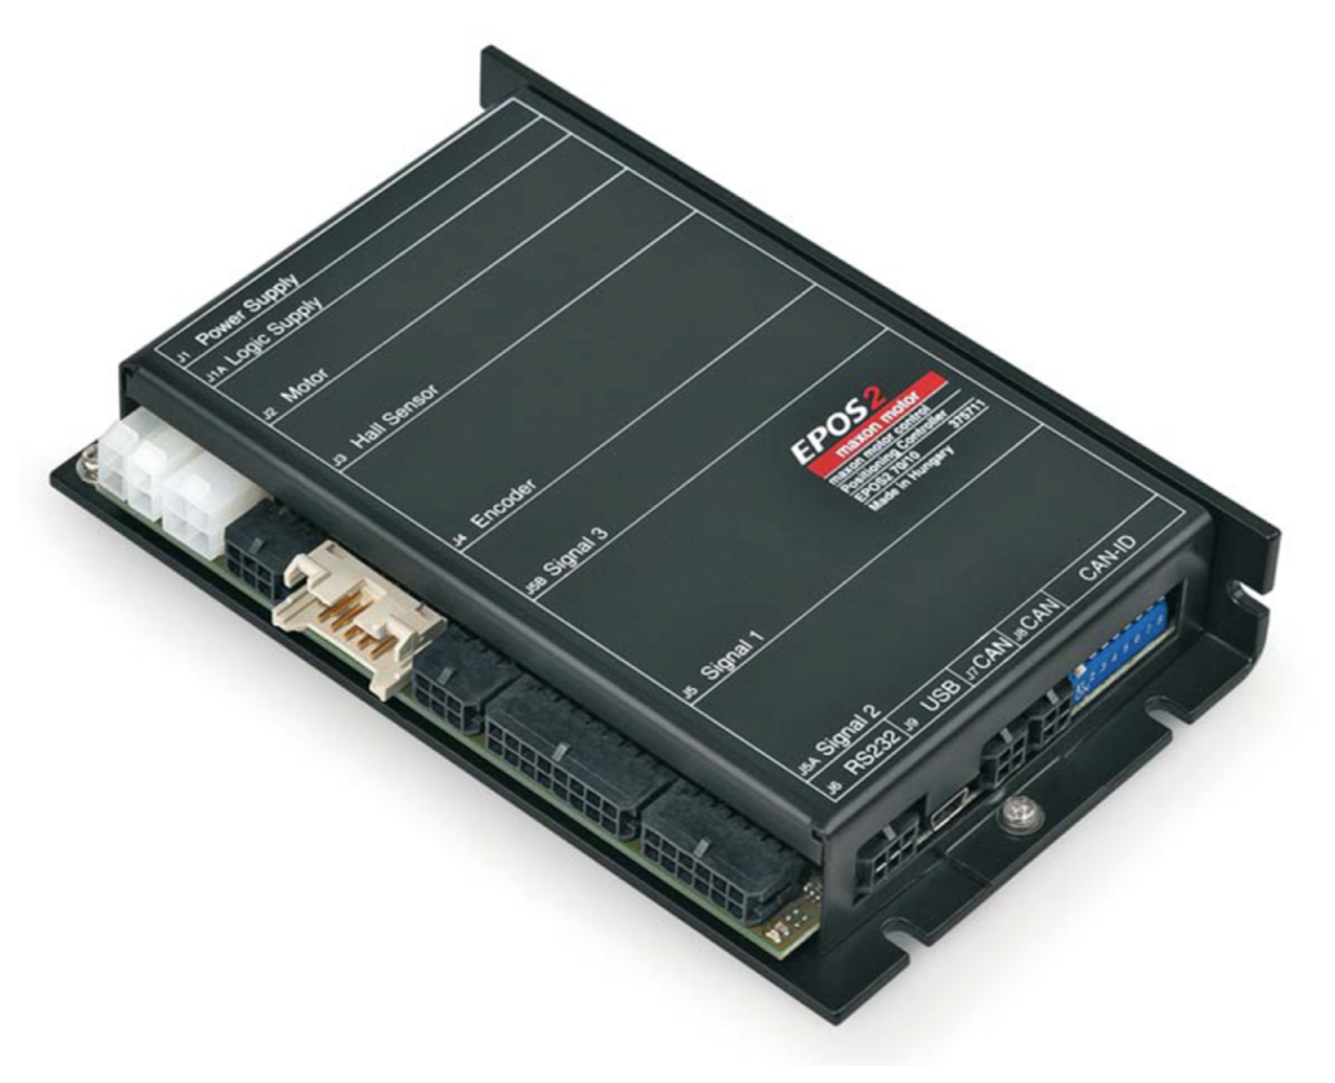
\includegraphics[height=40mm]{figure/epos.eps}
      \vspace*{3mm}
      \caption{EPOS2 70/10(375711)}
    \label{fig:epos}
    \end{center}
  \end{minipage}
  \begin{minipage}{0.6\textwidth}
      \begin{center}
	\makeatletter
	\def\@captype{table}
	\makeatother
	\caption{Specification of EPOS2 70/10(375711)}
	\label{tab:epos}
	\begin{tabular}{cc}\hline
	  power suppy voltage [VDC] & 11-70\\
	  Max output current [A] & 25\\
	  Max continuous current [A] & 10\\
	  Hall sensor & H1, H2, H3 \\
	  Encoder & A, A$\setminus$, B, B$\setminus$, I, I$\setminus$(max. 5MHz)\\
	  Analog Input & 2(differential, 12-bit, 0...+5 V)\\
	  RS232 & RxD; TxD(max. 115200 bit/2) \\\hline
	  \end{tabular}
	\end{center}
  \end{minipage}
\end{figure}

\vspace*{20mm}
\begin{figure}[htp]
  \begin{center}
    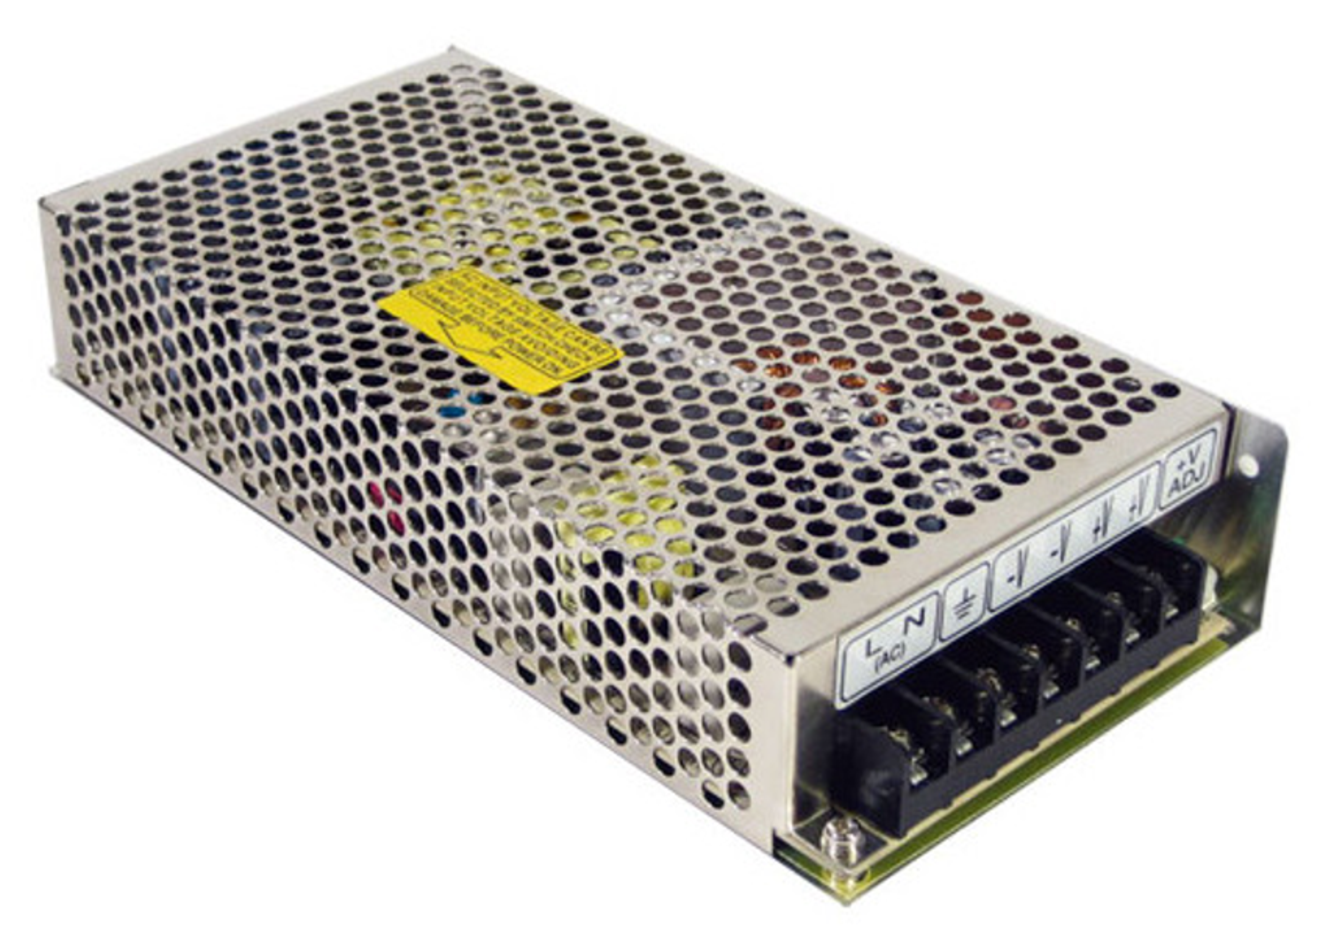
\includegraphics[height=40mm]{figure/rs_150_24.eps}
    \vspace*{3mm}
    \caption{Swiching Power Supply(RS-150-24)}
    \label{fig:rs_150_24}
  \end{center}
\end{figure}


\newpage
本研究では,シリアル通信を用いた位置制御を行った.

\newpage
\subsubsection{スライダクランク機構}
スライダクランク機構は回転運動を直進運動に変換する機構の一つである.図~\ref{fig:slider_crank}~に示すようにクランクとコネクティングロッドから構成される.本研究では路面の変位を$\pm 30mm$確保するためにクランク長は$r=45mm$,コネクティングロッドの長さは$l=90mm$とした.クランクの回転角$\theta_A$とコネクティングロッド先端の変位$x_0$の関係は式(~\ref{eq:mm_to_deg}~)で表される.本研究で行う試験では路面入力を行う為に入力を変位$x_0$,出力を回転角$\theta_A$とする関係式が必要である.しかし式(~\ref{eq:mm_to_deg}~)では計算が複雑である.そこでLook up tableを用いた.Look up tableは予め計算できるデータを配列として格納しておくことで,配列に対応する値を参照してデータを得ることができ,これにより計算の効率化を可能とする.使用したsimulinkブロックを図~\ref{fig:suspension}~に示す.本研究では.Lookuptableの配列データの数は91とした.配列の要素であるクランクの回転角$\theta_A$の範囲は$\pm45[^\circ ]$であり,$0.1[^\circ ]$刻みとした.また変位$x_0$は式(~\ref{eq:mm_to_deg}~)より計算した値となっている.

\begin{equation}
 \label{eq:mm_to_deg}
x_{0} =r\times \sin \theta _{A} +\sqrt{l^{2} -r^{2}\cos^{2} \theta _{A}} -\sqrt{l^{2} -r^{2}}
\end{equation}

\vspace*{5mm}
\begin{figure}[htp]
  \begin{center}
    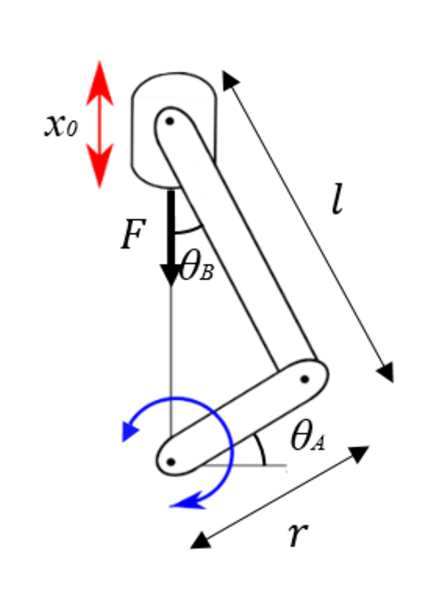
\includegraphics[height=50mm]{figure/slider_crank.eps}
    \vspace*{3mm}
    \caption{Slider Crank Mechanism}
    \label{fig:slider_crank}
  \end{center}
\end{figure}
% \vspace*{5mm}
% \begin{figure}[htp]
%   \begin{center}
%     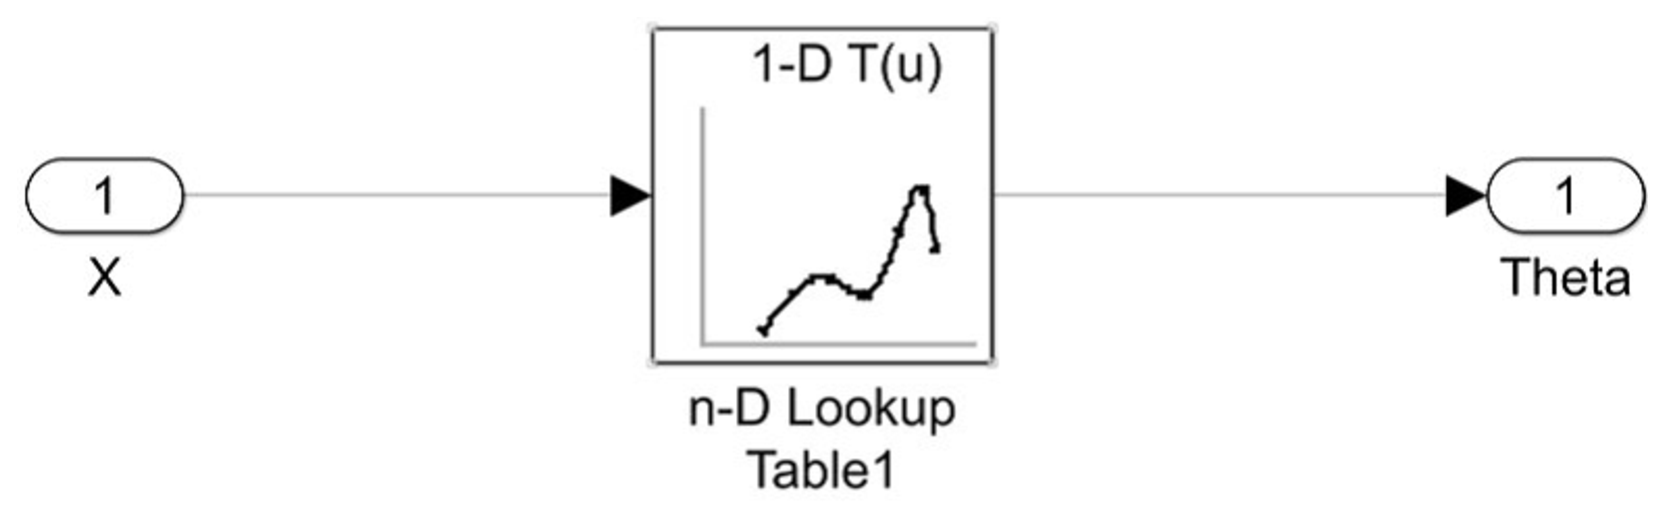
\includegraphics[height=30mm]{figure/Lookuptable.eps}
%     \vspace*{3mm}
%     \caption{Loou up table}
%     \label{fig:Look}
%   \end{center}
% \end{figure}

\newpage
\subsubsection{計測機器}
本試験ではダンパが発生させるサスペンションストロークを計測する.ここでは計測に用いるロードセルとレーザ変位計について説明する.

まず,ロードセルについて説明する.ダンパが発生する力の計測には図~\ref{fig:tclz-20na}に示す東京測器研究所の引張・圧縮型高精度荷重計「TCLS-20NA」を用いた.仕様を表~\ref{tab:tclz_20na}~に示す.このロードセルをダンパとばね上の間に取り付けることでダンパ力を計測する.ロードセルから出力された電圧値は,東京測器研究所のデジタル指示計「TD-96A」を用いて寒山する.このデジタル指示計は,ひずみゲージ式変換器を用いて荷重,変位,圧力などを測定できる.外観を図~\ref{fig:td_96a}~に,仕様を表~\ref{tab:td_96a}~に示す.


\vspace*{10mm}
\begin{figure}[h!]
  \begin{tabular}{cc}
  \begin{minipage}{0.5\hsize}
  \begin{center}
    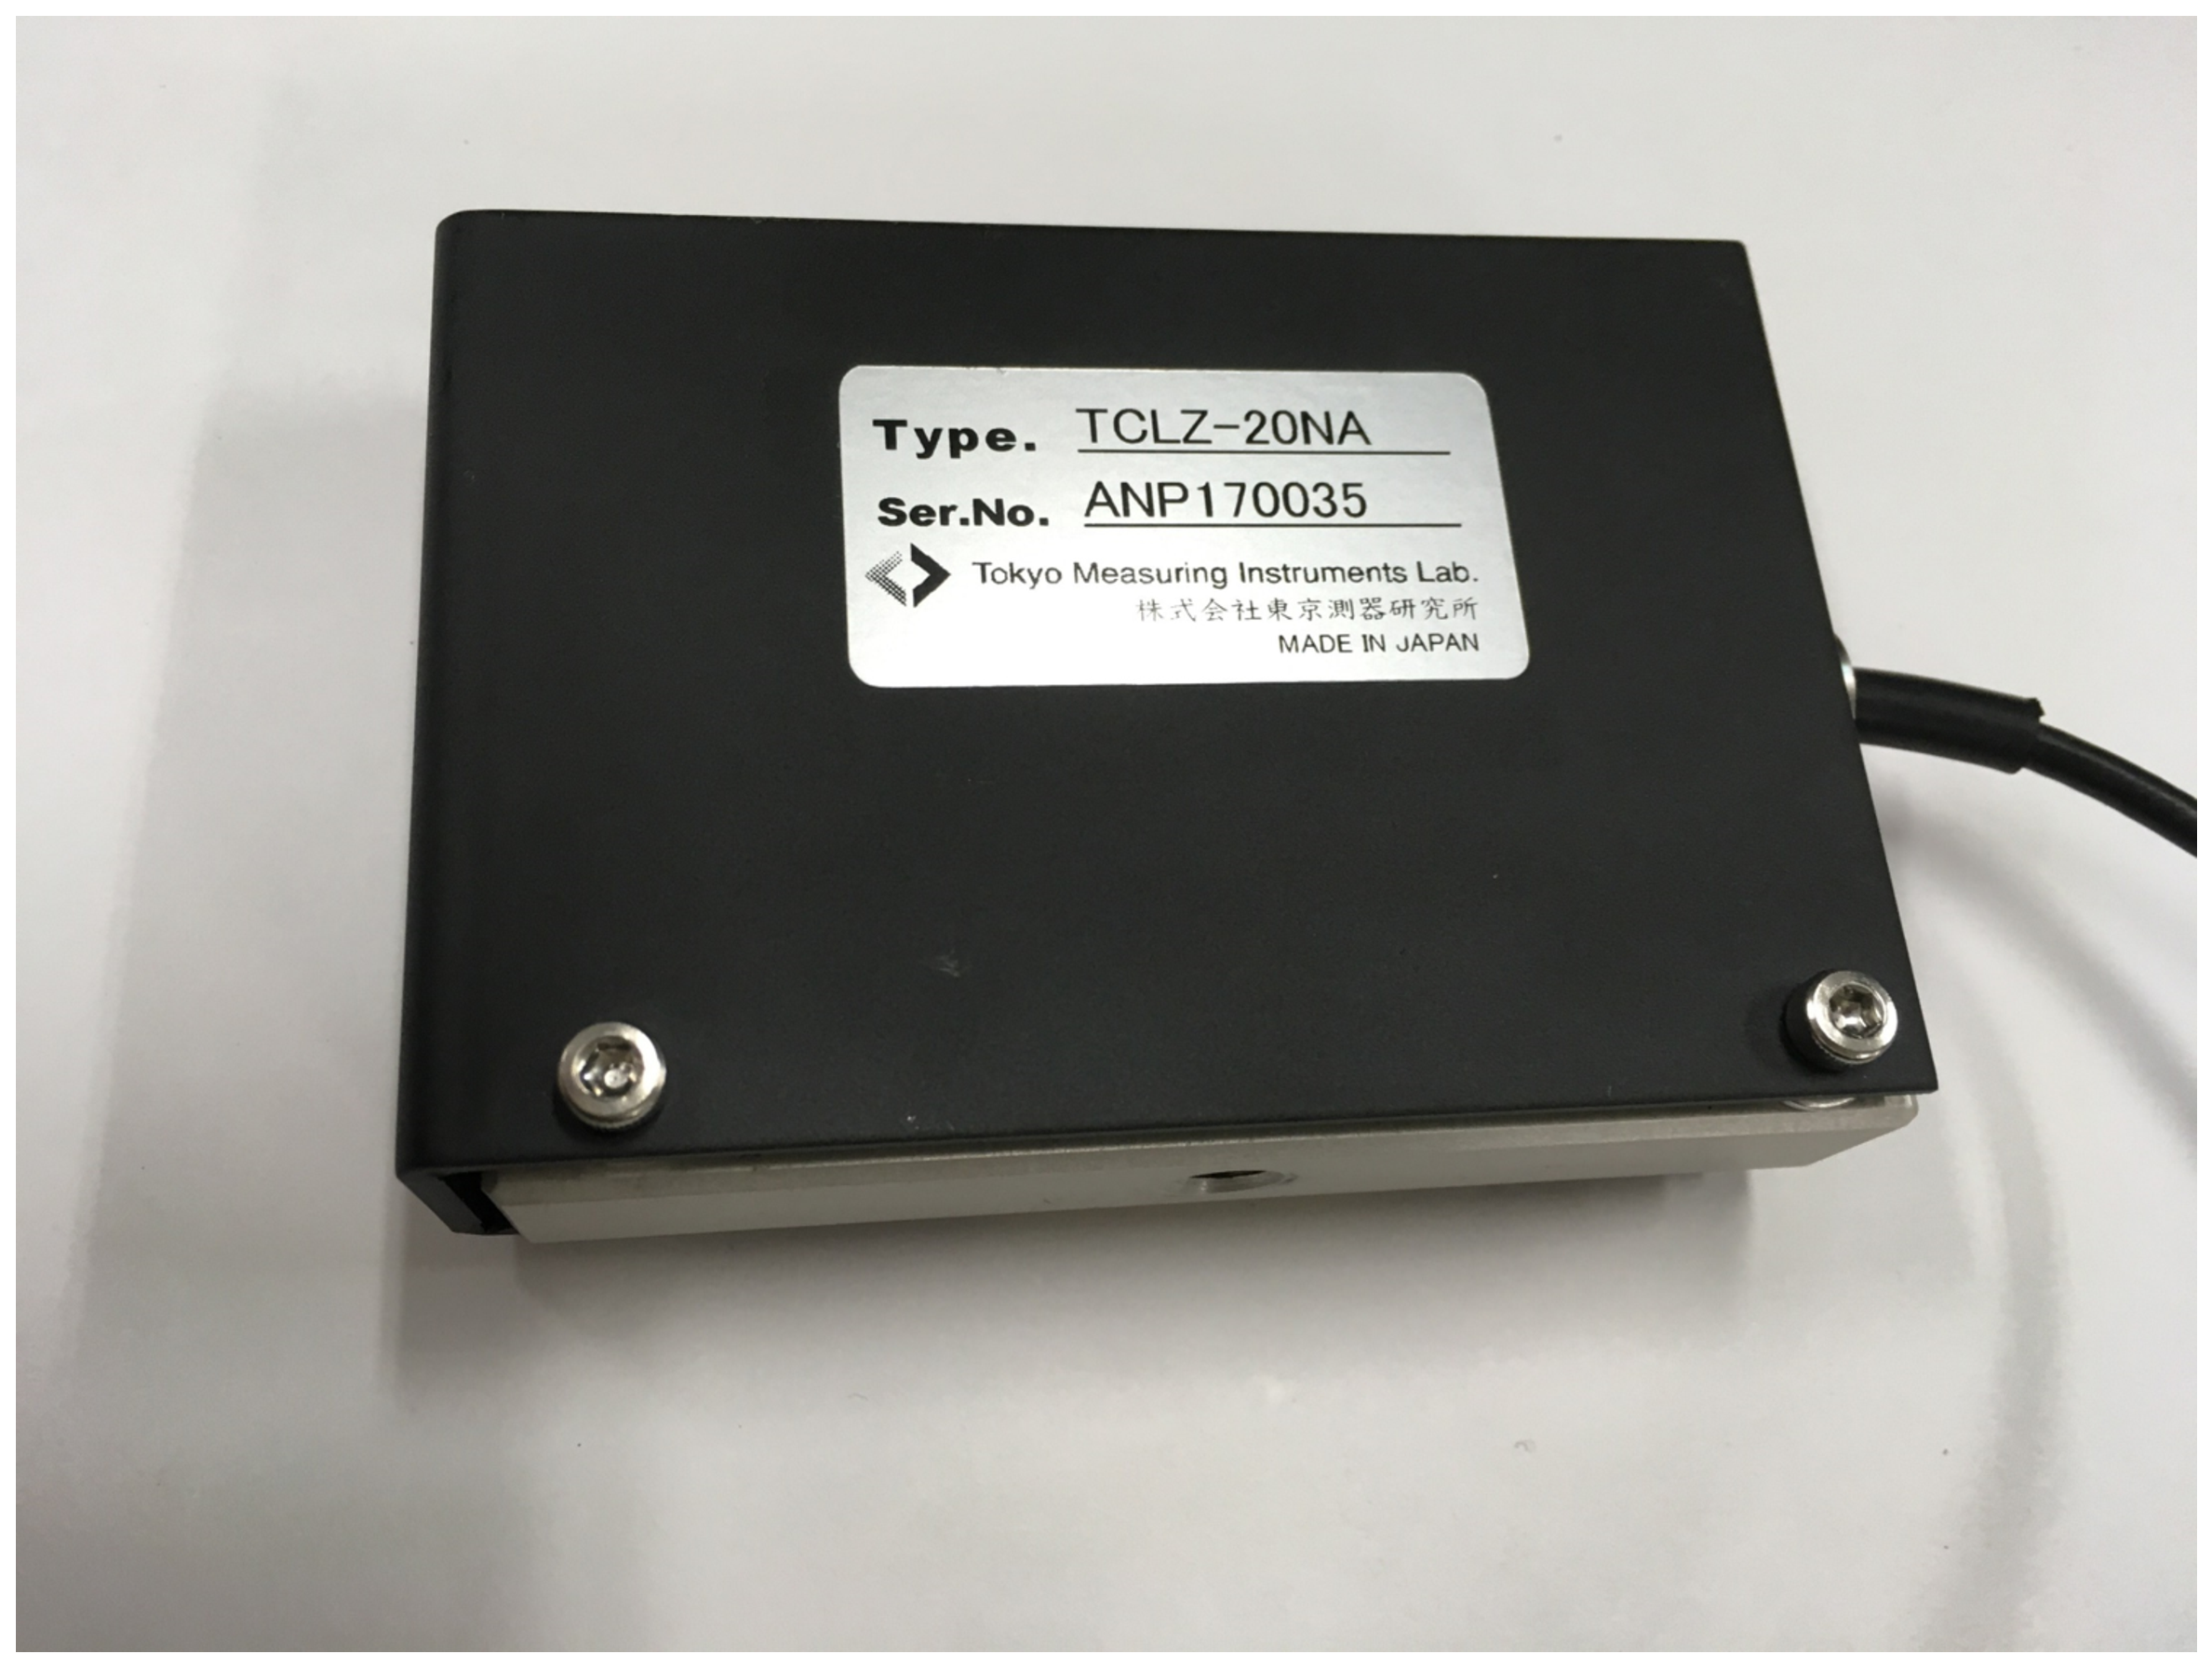
\includegraphics[height=40mm]{figure/tclz_20na.eps}
      \vspace*{3mm}
      \caption{Loadcell(TCLZ-20NA)}
      \label{fig:tclz-20na}
    \end{center}
  \end{minipage}
  \begin{minipage}{0.5\hsize}
     \begin{center}
      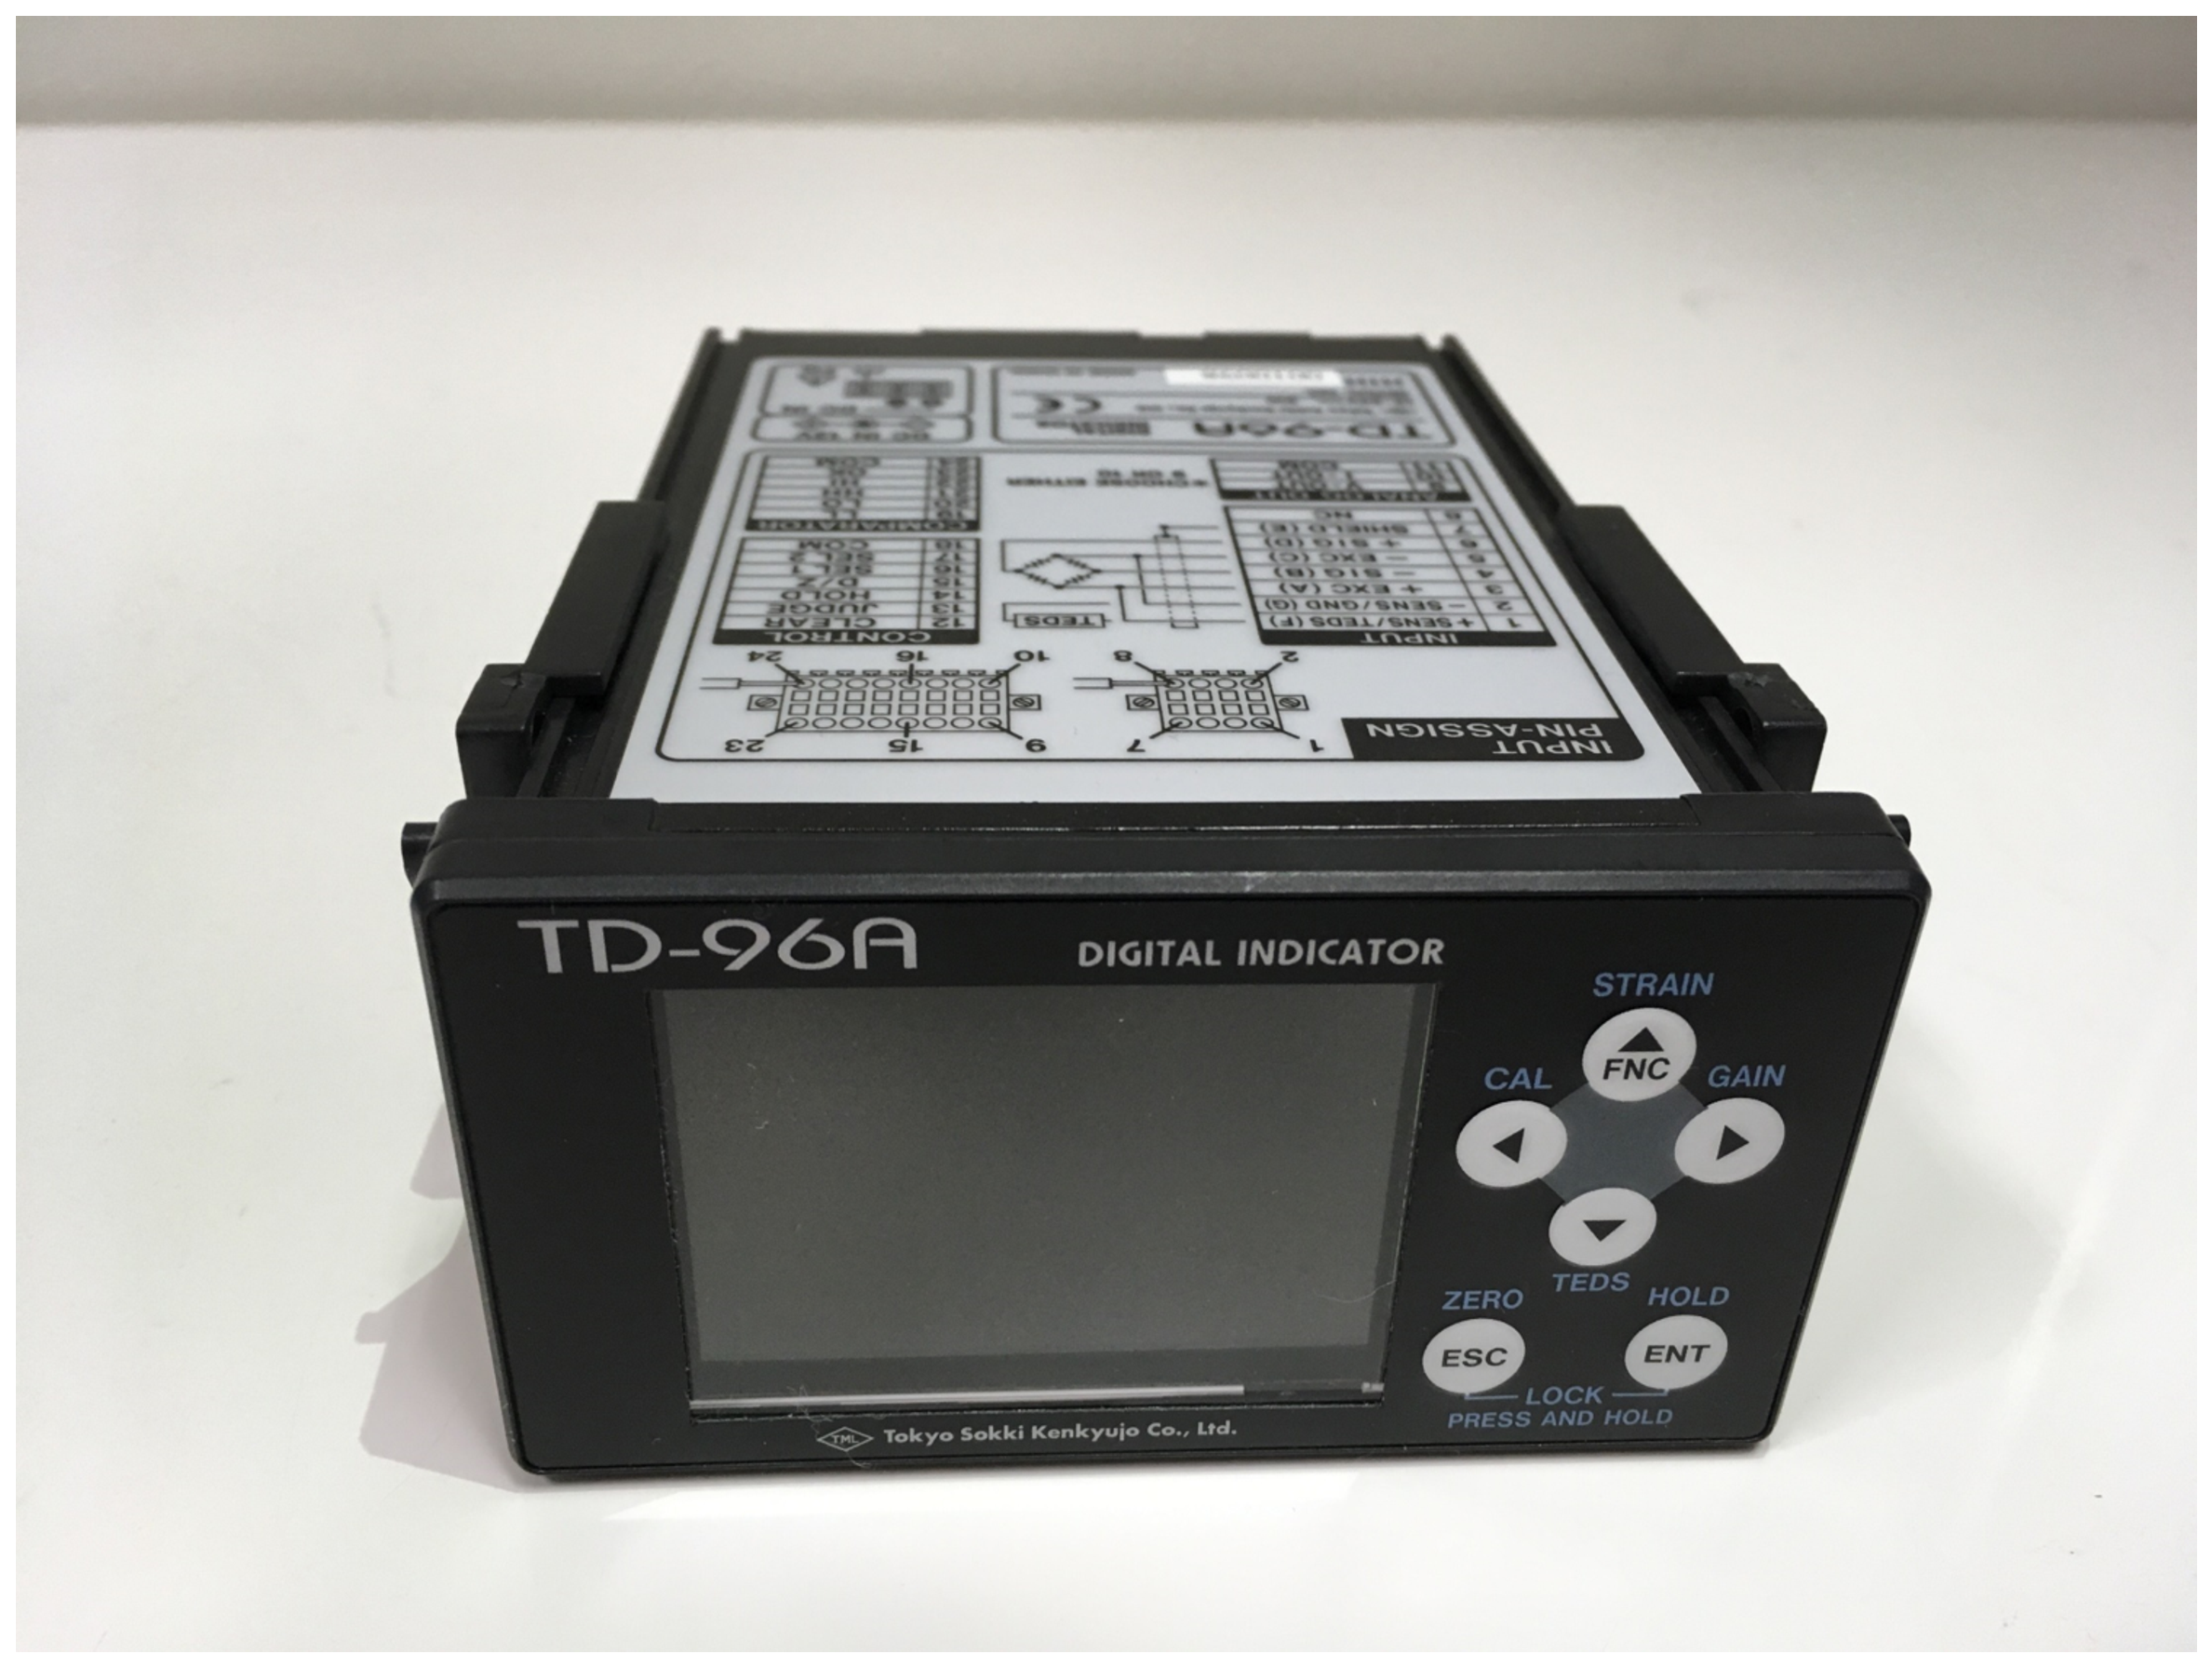
\includegraphics[height=40mm]{figure/td_96a.eps}
      \vspace*{3mm}
      \caption{Digital Indictor(TD-96A)}
      \label{fig:td_96a}
    \end{center}
  \end{minipage}
  \end{tabular}
 \end{figure}

\vspace*{10mm}
\begin{table}[h]
  \begin{center}
    \caption{Specification of Loadcell}
	\label{tab:tclz_20na}
	\begin{tabular}{crrc}\hline
	  Parameter & \multicolumn{2}{c}{Value}&\\\hline
	  Capacity & \multicolumn{2}{c}{20 N}&\\
	  Overload Capacity & \multicolumn{2}{c}{30N}&\\
	    & Ten.&Comp.\\
	  Rated Output & +1248.7 & -1248.4 & $\mu$V/V \\
	  Strain & +2497.3 & -2496.8 & $\times$ 10$^-6$ $\epsilon$ \\
	  Calibration Coefficient & 0.008009 & 0.008010 & N/1$\times$ 10$^-6$ \\\hline
	\end{tabular}
  \end{center}
\end{table}

\vspace*{10mm}
\begin{table}[h]
  \begin{center}
    \caption{Specification of TD-96A}
    \label{tab:td_96a}
    \begin{tabular}{cc}\hline
      Measurement Point & 1 \\
      Measurement Range [mV/V]& $\pm$3\\
      A/D Conversion Speed [Hz]& 4000\\
      D/A Output [mA]& 0$\pm$1$\sim\pm$10 V, 4$\sim$20\\
      Power supply & AC100 V 12 W, DC12$\sim$24 V 9 W \\\hline
    \end{tabular}
  \end{center}
\end{table}

\newpage
つづいてレーザ変位計について説明する.サスペンションストロークの計測には図~\ref{fig:il_300}~に示す株式会社KEYENCEのセンサヘッド「IL-300」を用いた.仕様を表~\ref{tab:il_300}~に示す.出力電圧は$\pm 5V,1-5V,0-5V$から選択できる.計測距離を$L[mm]$,アナログ出力電圧を$V[V]$としたとき,寒山式はそれぞれ以下の式のようになる.本研究では出力電圧$\pm 5V$の式(~\ref{eq:v5}~)を用いた.また,アンプとして,図~\ref{fig:il_1500}にに示す株式会社KEYENCEのアンプユニット「IL-100」を用いた.アンプユニットには,図~\ref{fig:lxo18_2a}~に示す定電圧/定電流直流電源「LXO18-2A」を用いて12Vをアンプユニットに供給している.

\begin{eqnarray}
 \label{eq:v5} L &=& V_{\pm5V} \times 28\\
 \label{eq:v15} L &=& V_{1-5V} \times 70\\
 \label{eq:v05} L &=& V_{0-5V} \times 56
\end{eqnarray}

\vspace*{10mm}
\begin{figure}[htp]
  \begin{minipage}{0.3\textwidth}
    \begin{center}
      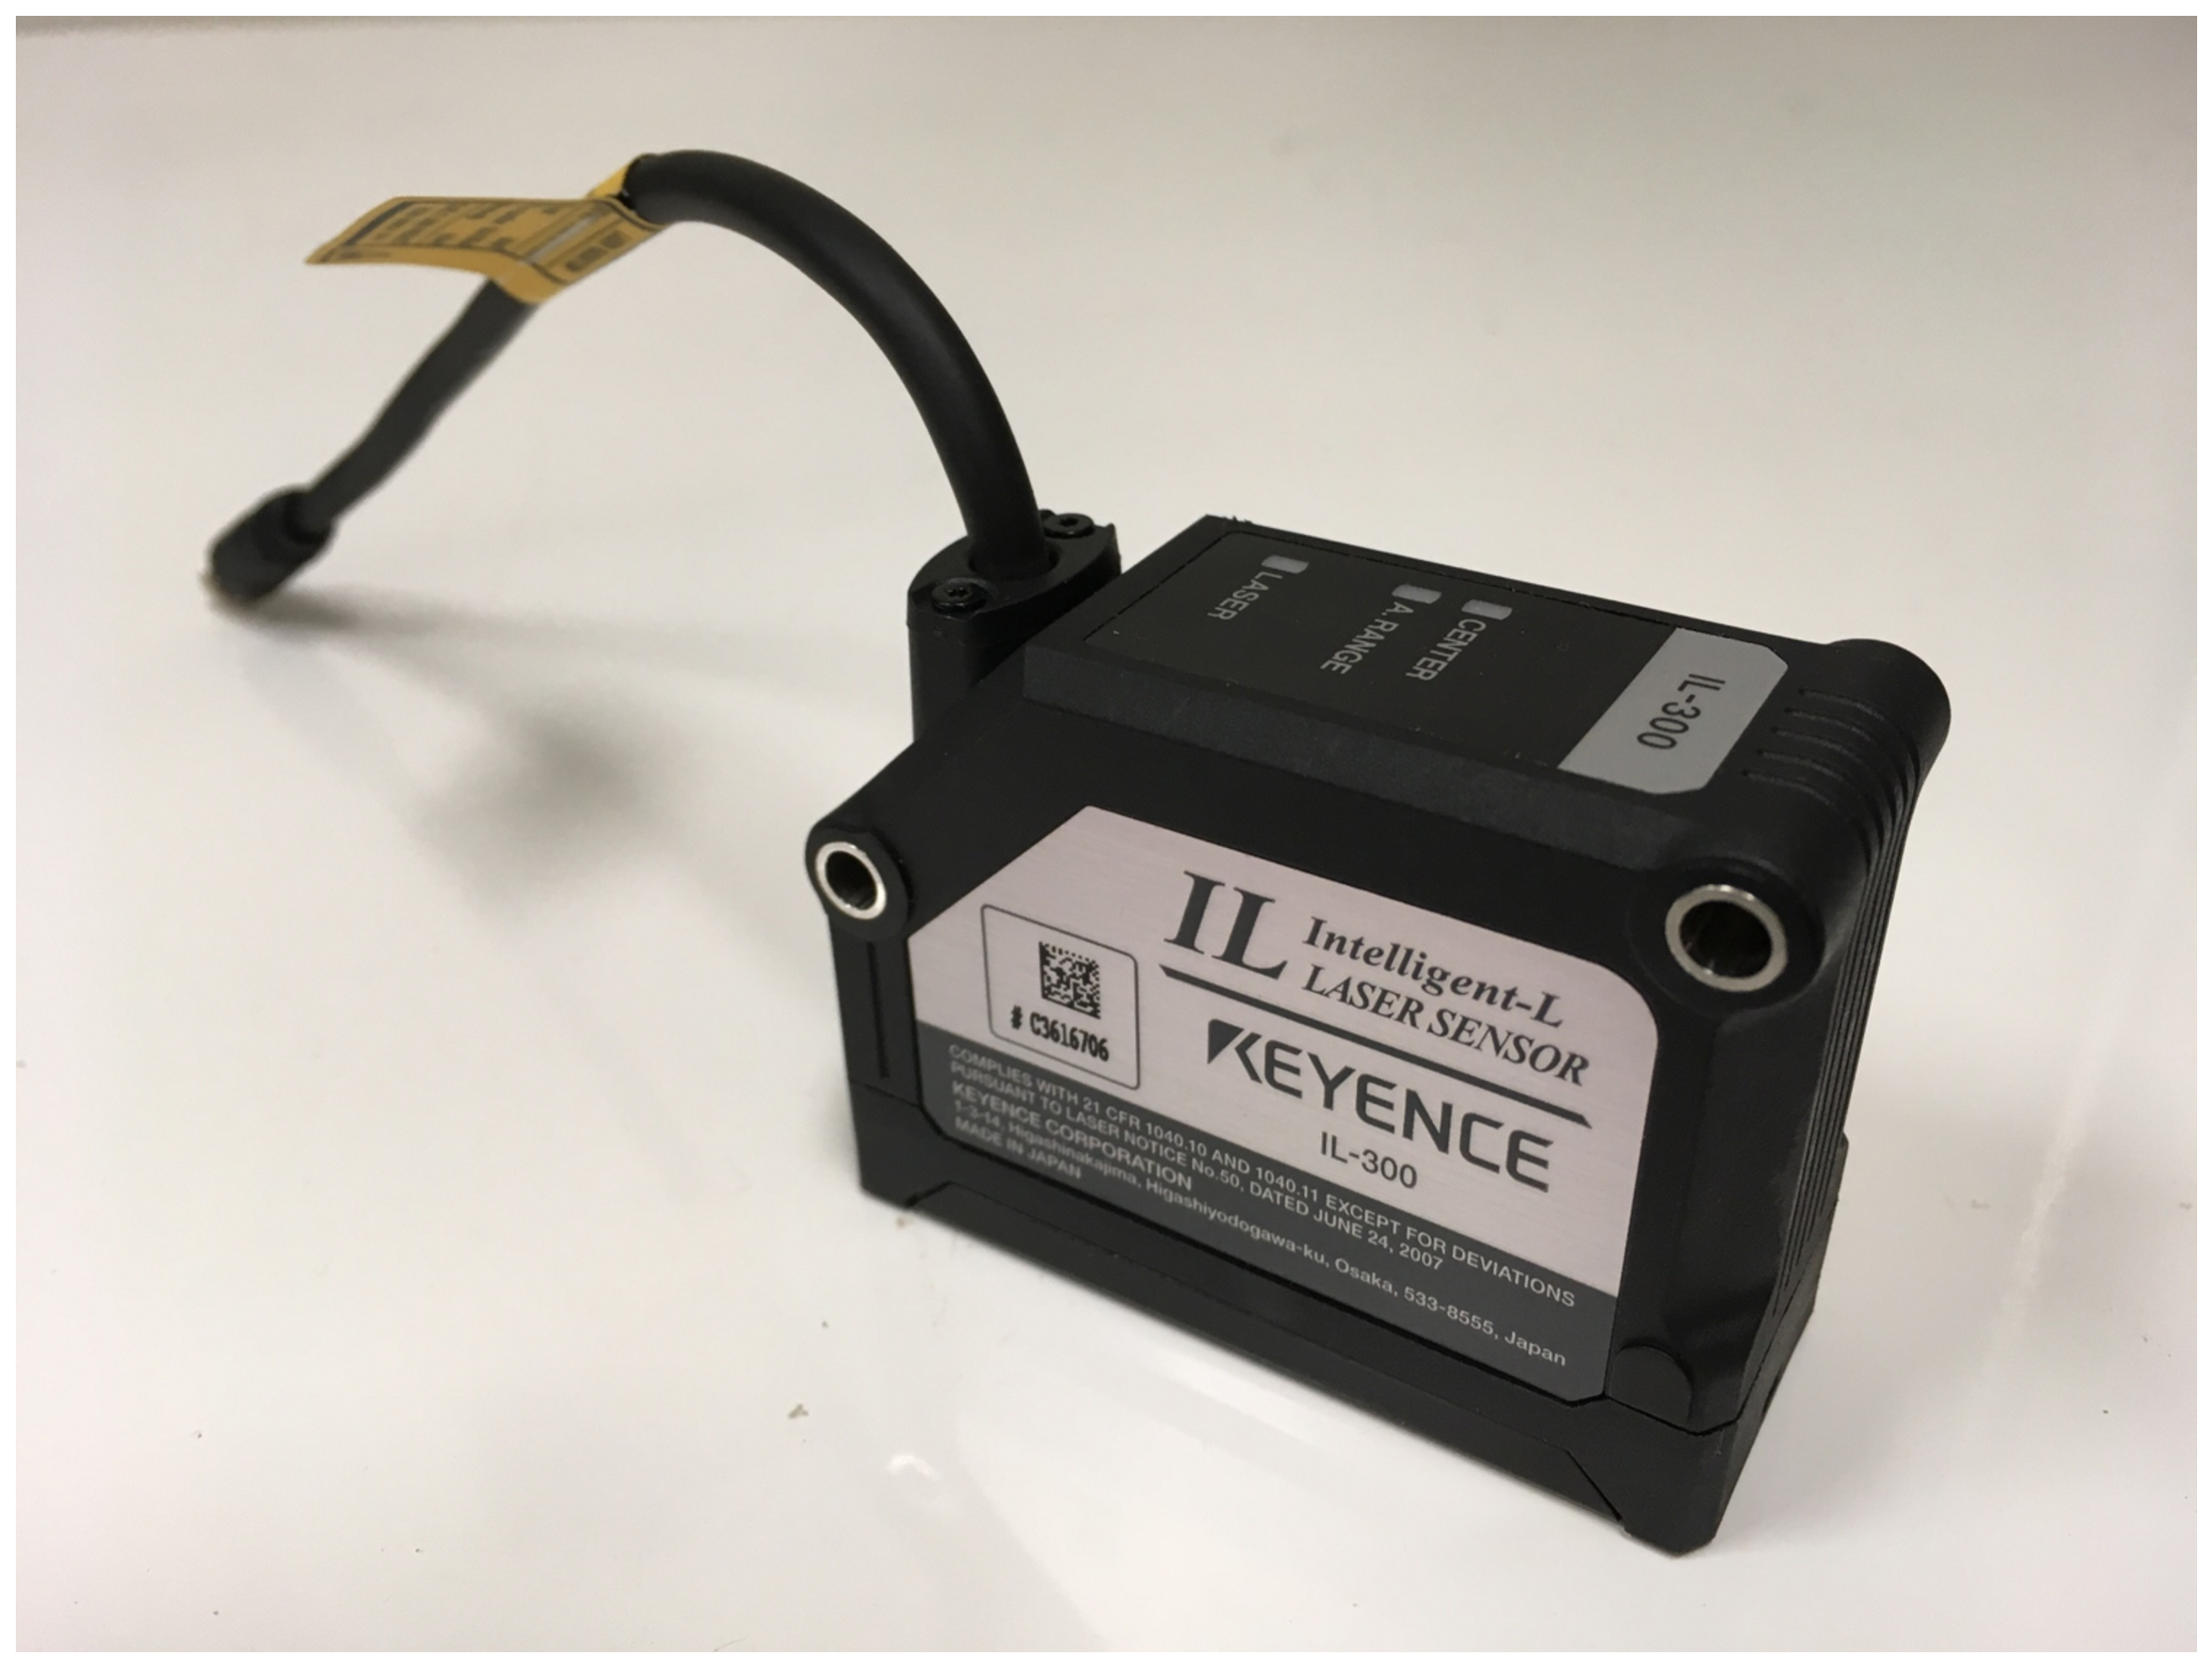
\includegraphics[height=40mm]{figure/il_300.eps}
      \vspace*{3mm}
      \caption{Laser Displacement Sensor(IL-300)}
      \label{fig:il_300}
    \end{center}
  \end{minipage}
  \begin{minipage}{0.7\textwidth}
      \begin{center}
	\makeatletter
	\def\@captype{table}
	\makeatother
	\caption{Specification of Laser Displacement Sensor}
	\label{tab:il_300}
	\begin{tabular}{ccc}\hline
	  Measurement Center Distance [mm] & 300\\
	  Measuring Range & 160-450 mm\\
	  Sampling Period [$\mu$s]& 0.33 / 1 / 2 / 5\\
	  Resolition [$\mu$m] & 10\\
	  Linearity [\%F.S.] & $\pm$0.25\\
	  Receiving Element & Liner Image Sensor\\
	  Resistance to Vibration [Hz] & 10-55\\
	  Laser Class & 2\\
	  Power Supply & DC10-30 V\\\hline
	  \end{tabular}
	\end{center}
  \end{minipage}
\end{figure}

\vspace*{10mm}
\begin{figure}[htp]
  \begin{minipage}{0.5\textwidth}
    \begin{center}
      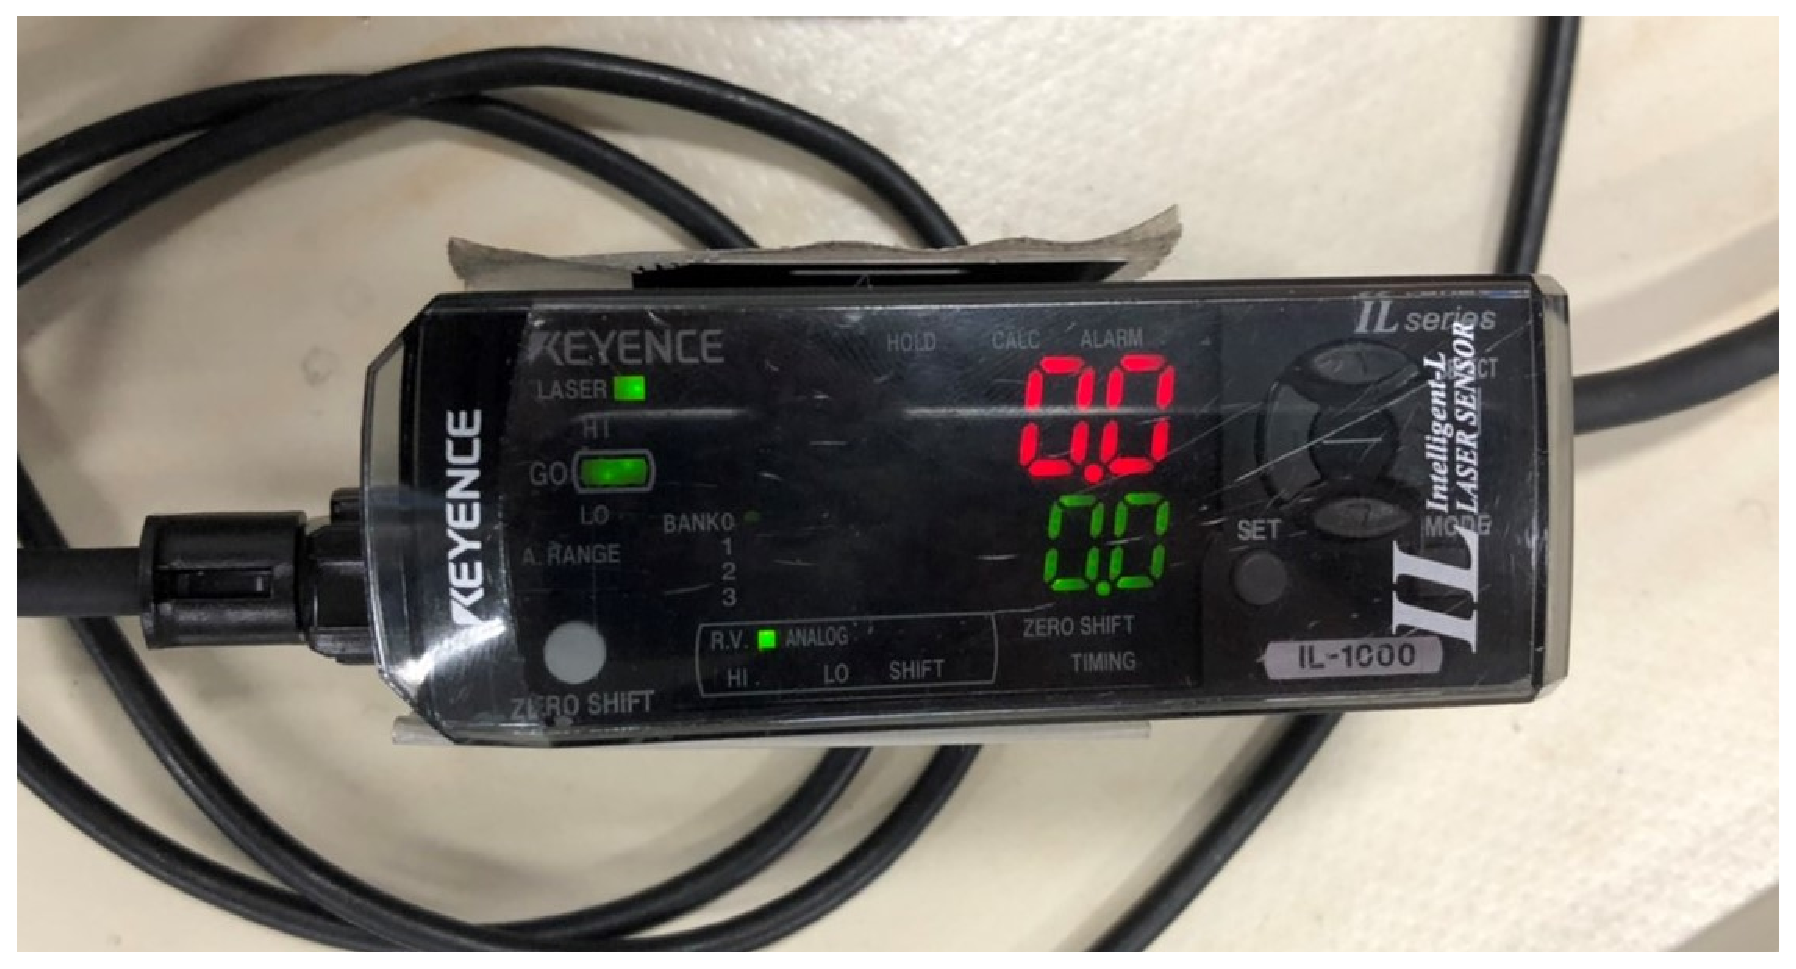
\includegraphics[height=40mm]{figure/amp.eps}
      \vspace*{3mm}
      \caption{Amplifier Unit(IL-1000)}
      \label{fig:il_1500}
    \end{center}
  \end{minipage}
  \begin{minipage}{0.5\textwidth}
    \begin{center}
      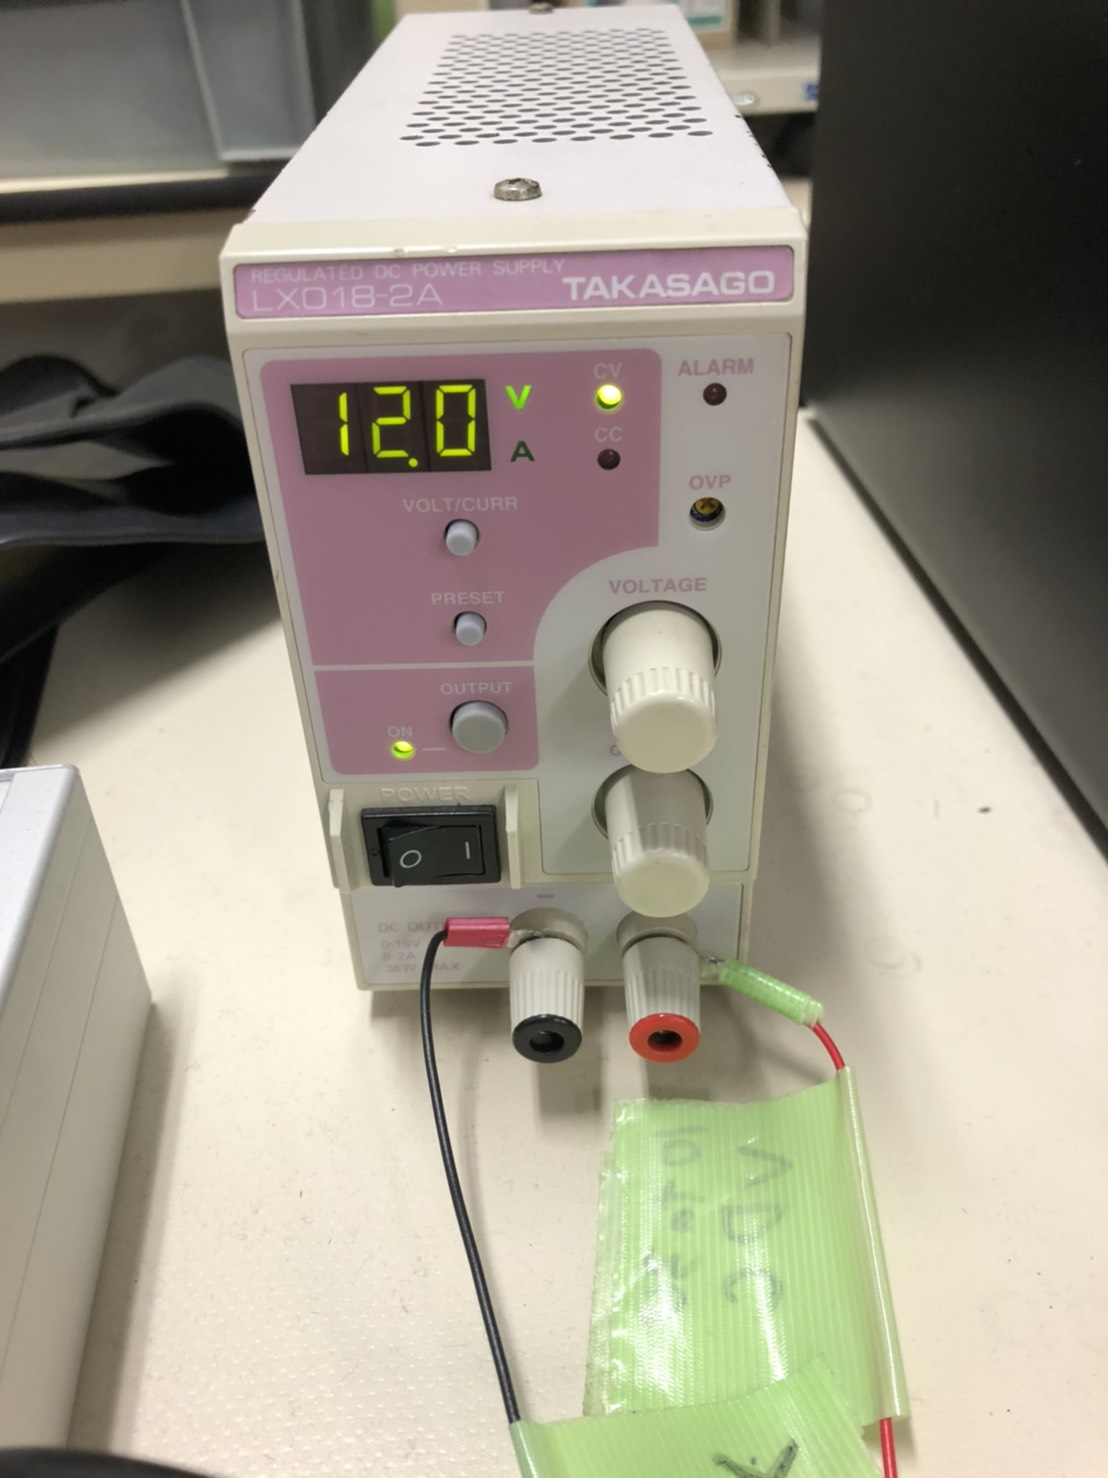
\includegraphics[height=40mm]{figure/power_supply.eps}
      \vspace*{3mm}
      \caption{Power Supply Unit(LXO18-2A)}
      \label{fig:lxo18_2a}
    \end{center}
  \end{minipage}
\end{figure}

\subsection{ソフトウェア部}
\subsubsection{dSPACEシステム}
本システムでは,dSPACE社製の開発環境であるdSPACEシステムを利用している.上下変位計算とハードウェア制御にはdSPACE社製のController Board「DS1104 Controller Board」を使用している.Controller Boardを図~\ref{fig:ds1104}に,Connector Panelを図~\ref{fig:conpane}に示す.Controller Boardは,デジタル入出力用チャンネル,A/Dコンバータ用チャンネル,D/Aコンバータ用チャンネルによるエンコーダの計測や,Serial Interfaceに対応しておりボーレート最大115200bpsのRS232通信が可能である.

\vspace{10mm}
\begin{figure}[h]
    \begin{tabular}{c}
      \begin{minipage}{0.5\hsize}
	\begin{center}
	  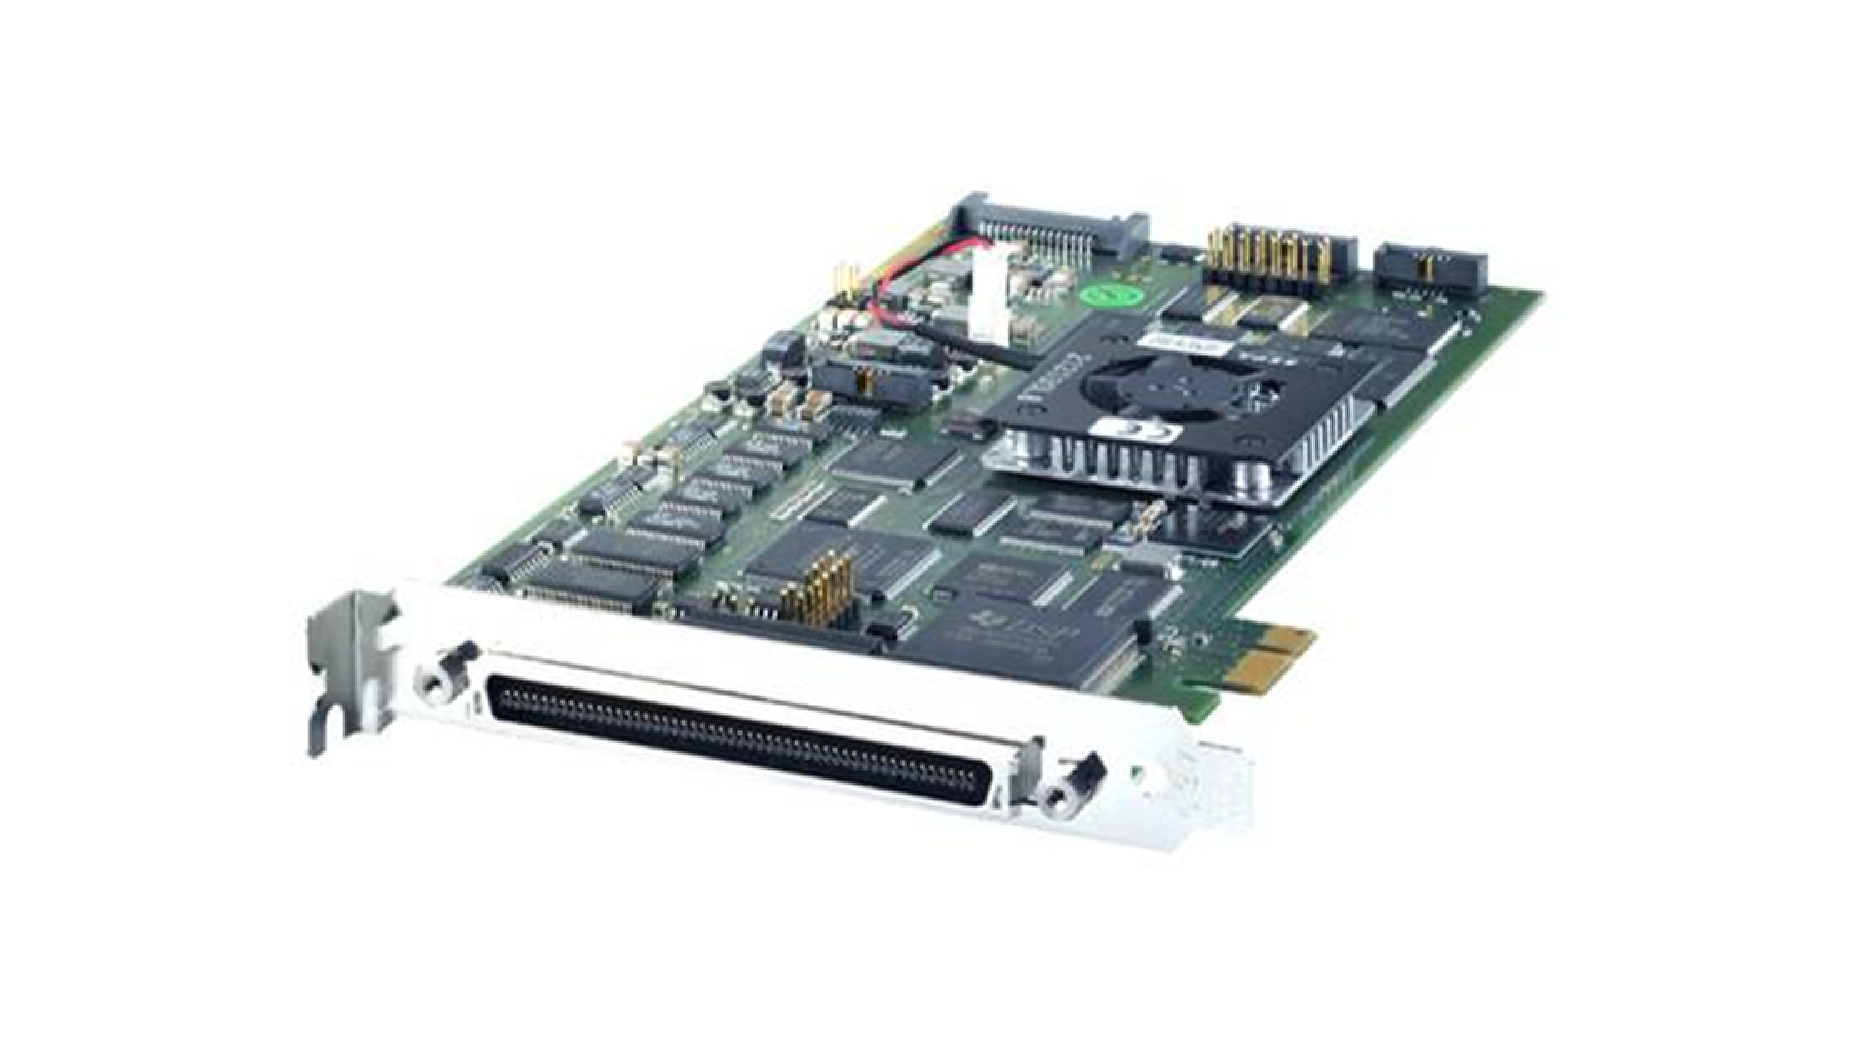
\includegraphics[height=25mm]{figure/ds1104.eps}
	  \caption{Controller Borad\cite{dspace}}
	  \label{fig:ds1104}
	\end{center}
      \end{minipage}
      \begin{minipage}{0.5\hsize}
	\begin{center}
	  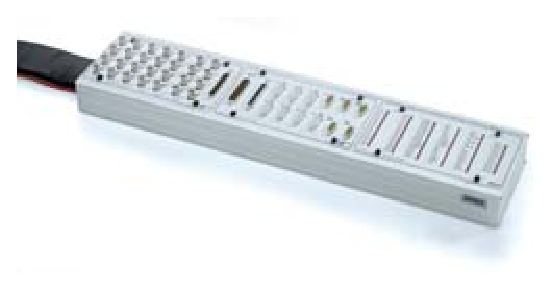
\includegraphics[height=25mm]{figure/conpane.eps}
	  \caption{Connector Panel\cite{dspace}}
	  \label{fig:conpane}
	\end{center}
      \end{minipage}
    \end{tabular}
\end{figure}

Real-Time Interfaceは,dSPACE社製のハードウェアとMathWorks社製のソフトウェア「MATLAB/Simulink」の間のリンクとなるものである.これにより,Simulinkモデルを用いてdSPACEシステムの入出力機器と信号処理を行うことができる.また,MATLAB/Simulinkで作成されたモデルは,Simulink Corderにより,実時間で実行可能なCコードに変換され,Controller Board上で実行される.このような開発環境を構築することで,実時間シミュレーションを行うHILSシステムを実現している.制御インターフェースとしては,dSPACE社生のControl Deskを用いている.「MATLAB/Simulink」と関連付けることで,試験条件の設定やハードウェアへの指令値,計測値,車両運動解析の結果をモニタリングできる.また,リアルタイムで計測値や解析結果をグラフとして描画できる.図\ref{fig:contrl_desk}では指令値や計測値,上下変位計算の結果を表示したControl Deskの画面である.

\vspace{10mm}
\begin{figure}[h]
 \centering
 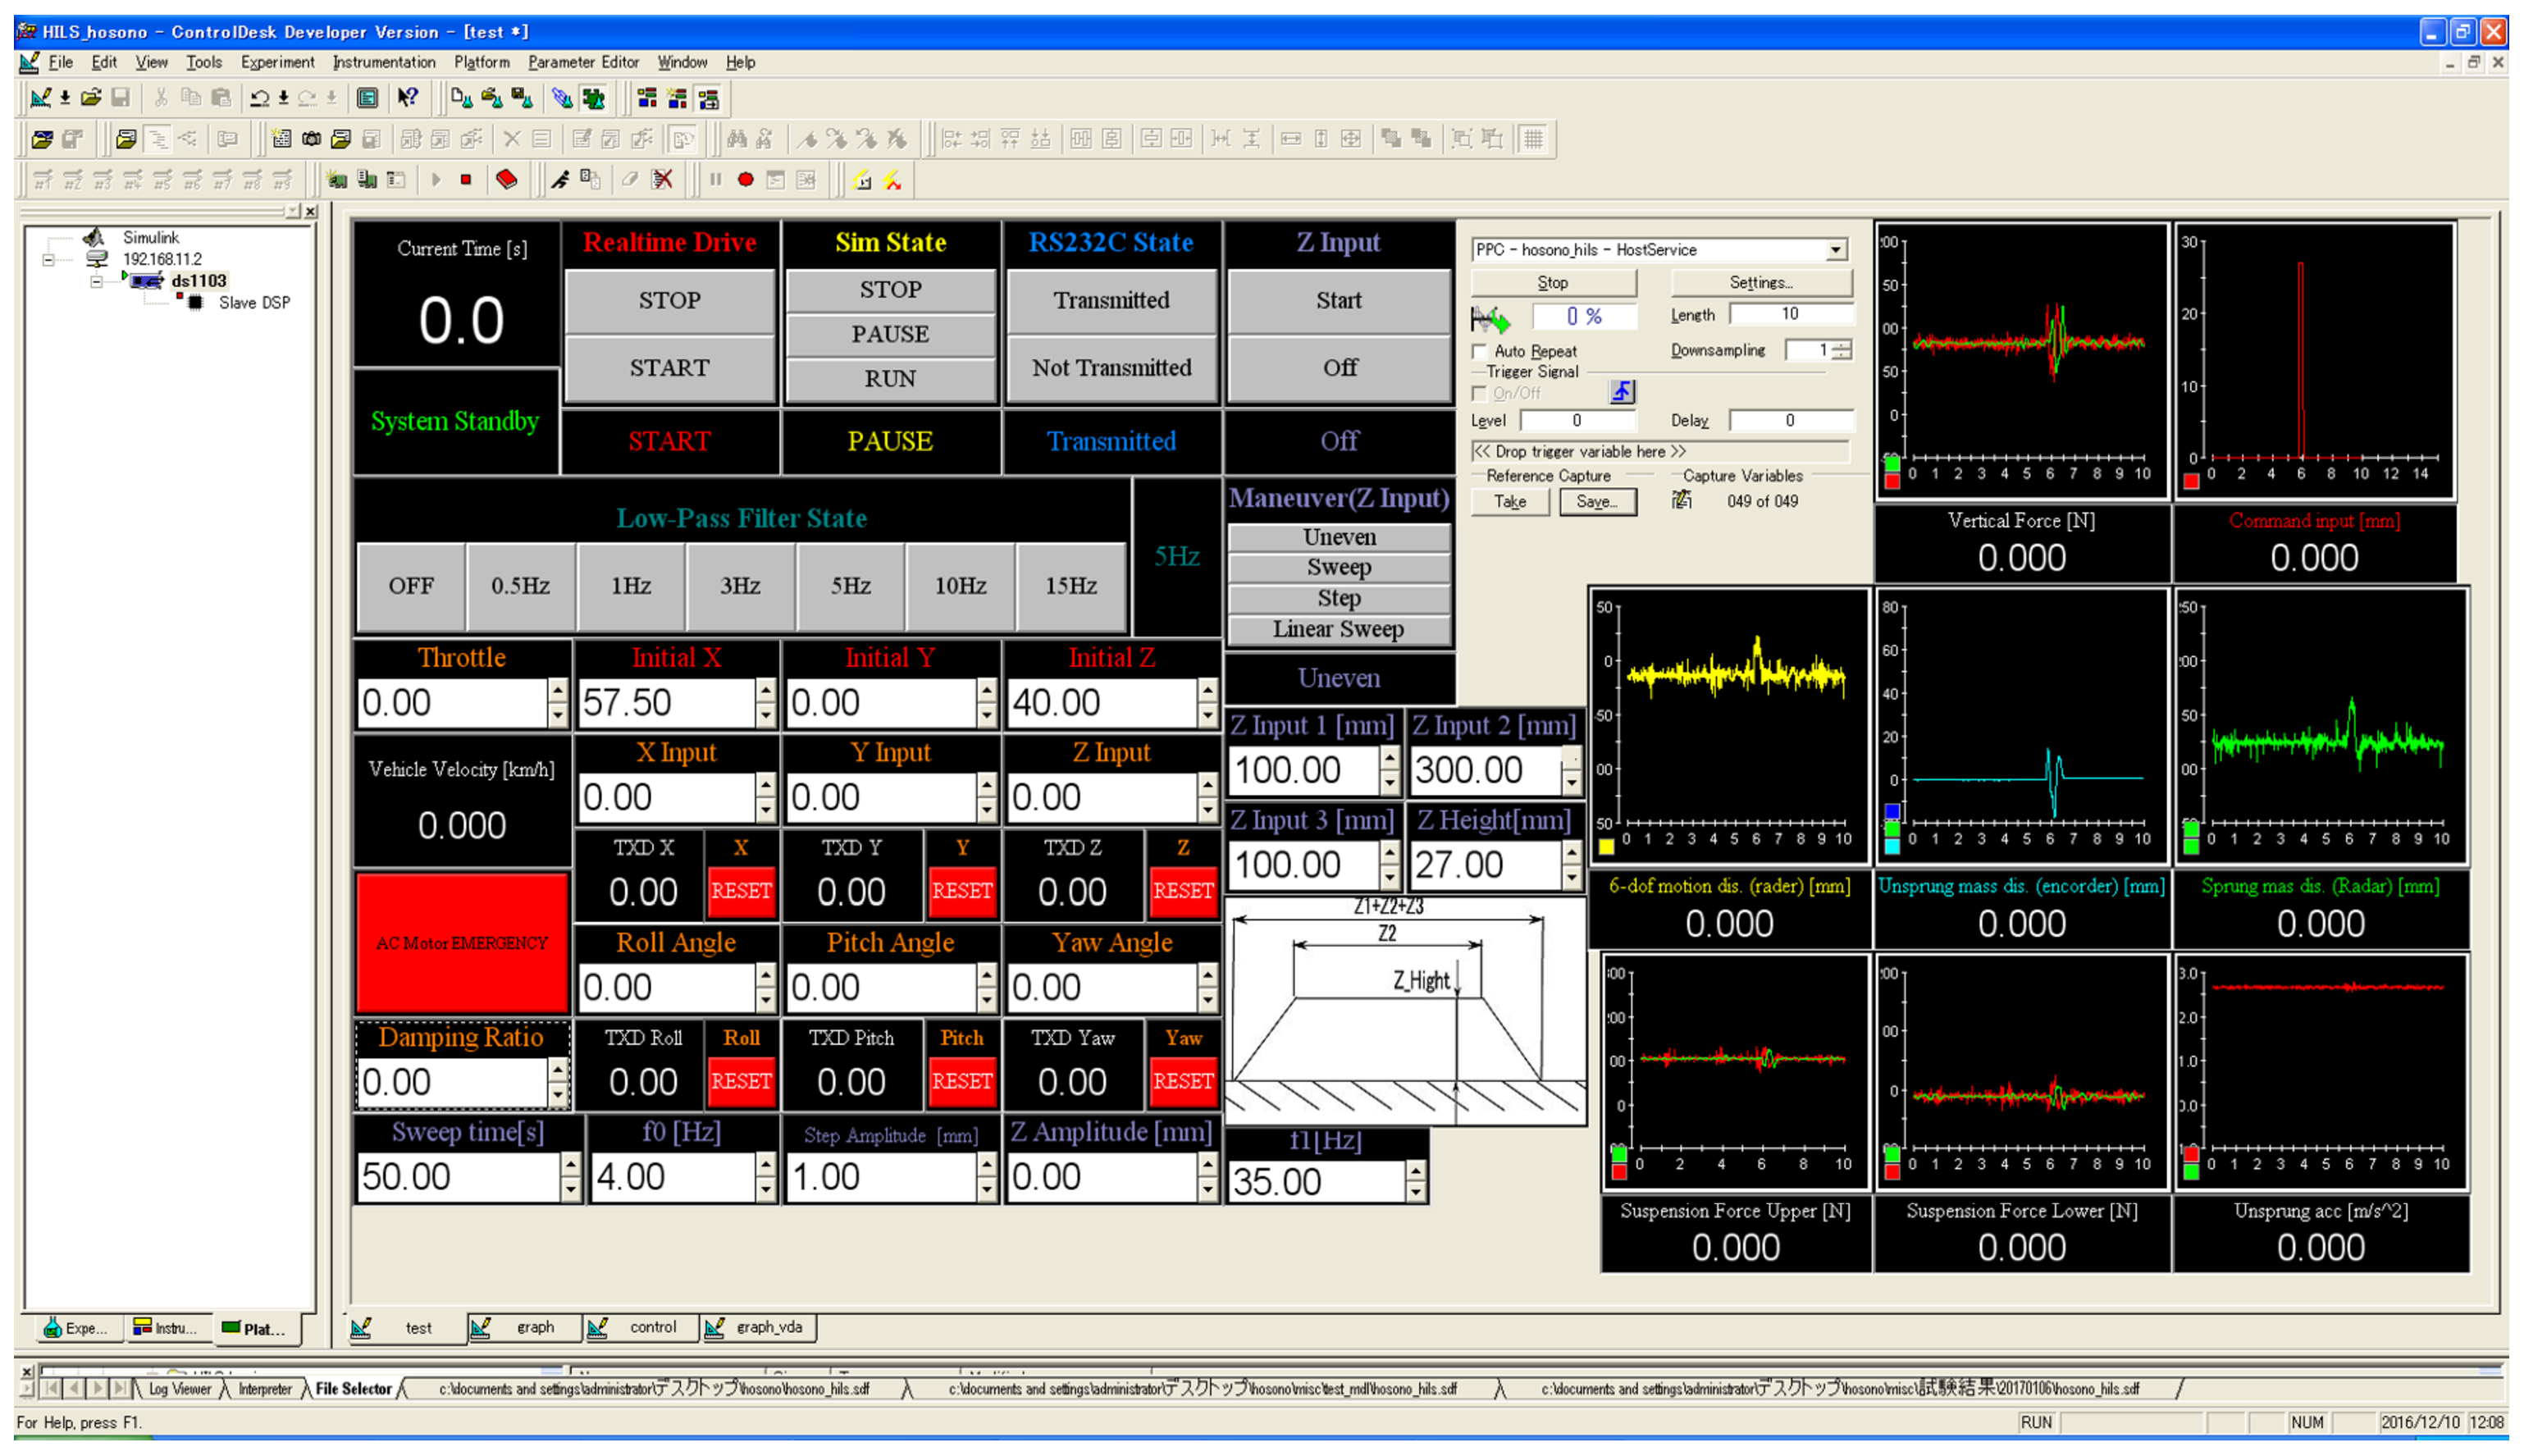
\includegraphics[height=50mm]{figure/control_desk.eps}
 \vspace{2mm}
  \caption{Control Desk}
 \label{fig:control_desk}
\end{figure}

\newpage
\subsubsection{解析モデル}
本システムにおいて解析モデルは上下2自由度モデルを用いた.上下2自由度モデルは車両の上下動を表すことのできるモデルの一つである\cite{carbody_model}.モデル図を図~\ref{fig:analysis_model}に,諸元を表~\ref{tab:carbody_parameter}に示す.また,このモデルの運動方程式は以下のとおりである.

\begin{eqnarray}
 \label{eq:2dof_m1} &&m_1\ddot x_1 + k_1(x_1-x_0) + k_2(x_1-x_2) - f_c = 0\\
 \label{eq:2dof_m2} &&m_2\ddot x_2 + k_2(x_2-x_1) + f_c = 0
\end{eqnarray}

ここで,$m_1$はばね下質量 ,$m_2$はばね上質量,$k_1$,$k_2$はばね定数,$f_c$はダンパ力,$x_0$は路面変位,$x_1$はばね下変位,$x_2$はばね上変位である

\vspace{10mm}
ここで,$m_1$はばね下質量 ,$m_2$はばね上質量,$k_1$,$k_2$はばね定数,$c_2$は減衰係数,$x_0$は路面変位,$x_1$はばね下変位,$x_2$はばね上変位である.そして,$f_c$はHILS試験機で計測されたダンパ力を用いる.

\vspace*{10mm}
\begin{figure}[htp]
  \begin{minipage}{0.5\textwidth}
    \begin{center}
      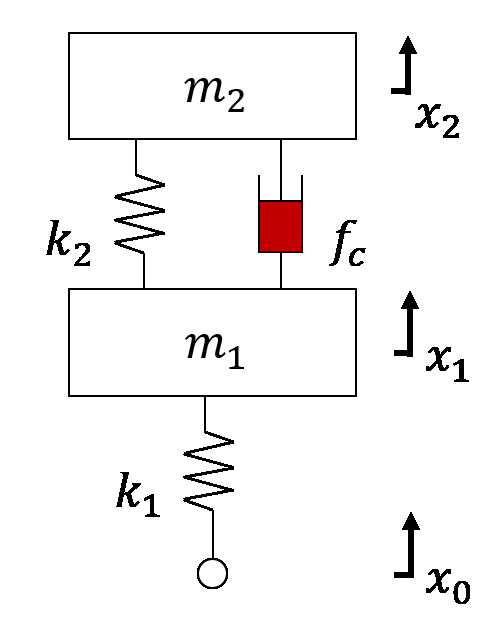
\includegraphics[height=40mm]{figure/analysis_model.eps}
      \vspace*{3mm}
      \caption{Analysis Model}
      \label{fig:analysis_model}
    \end{center}
  \end{minipage}
  \begin{minipage}{0.5\textwidth}
      \begin{center}
	\makeatletter
	\def\@captype{table}
	\makeatother
	\caption{Parameter of Analysis Model}
	\label{tab:carbody_parameter}
	  \begin{tabular}{cc}\hline
	    Unsprung Mass $m_1$ [kg] & 1.5\\
	    Sprung Mass $m_2$ [kg] & 6.9\\
	    Spring constant $k_1$ [N/m] & 2200\\
	    Spring constant $k_2$ [N/m] & 439\\\hline
	  \end{tabular}
	\end{center}
  \end{minipage}
\end{figure}

\newpage
\section{アクチュエータの制御手法}
本研究で用いるアクチュエータの制御手法について説明する.アクチュエータへの入力$\bar{x_0}$は解析モデルの結果に基づいて決定される.ここで解析モデルは上下2自由度振動系であるのに対し,本研究で用いるHILS試験機はばね上が固定された1自由度振動系である.2自由度振動系の上下変位$x_2-x_1$は,1自由度振動系の$-\bar{x_1}$に対応する.自由度が異なるため,解析モデルの入力である路面変位$x_0$をHILS試験機のアクチュエータの入力$\bar{x_0}$にすることはできない.そのため,路面変位を解析モデルへ入力し,計算された上下変位$x_2-x_1$と試験機の$x-\bar{x_1}$が一致するようにアクチュエータを制御する.HILSシステムのブロック線図を図~\ref{fig:block_diagram}~に示す.

%------- block diagram -------------
\vspace*{7mm}
\begin{figure}[htp]
  \begin{center}
    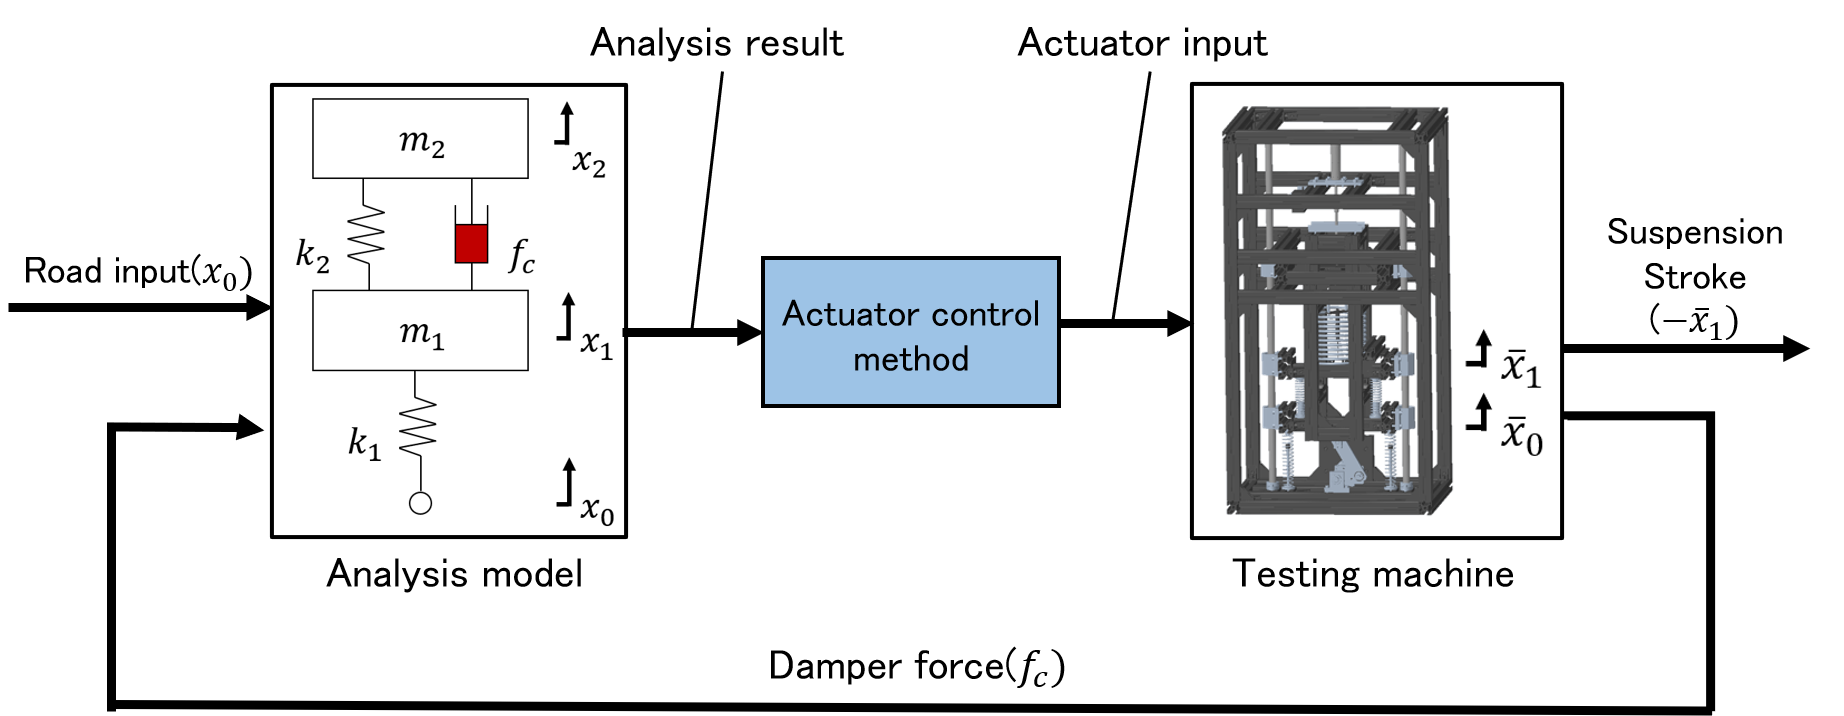
\includegraphics[height=40mm]{figure/block_diagram.eps}
    \vspace*{3mm}
    \caption{Block diagram of HILS system}
    \label{fig:block_diagram}
  \end{center}
\end{figure}

\subsection{相対変位を用いた制御手法}
アクチュエータの制御手法として相対変位を用いた手法について説明する.解析モデルとHILS試験機の自由度の違いにより,アクチュエータへの入力$\bar{x_0}$は解析モデルの車体-路面間の相対変位$x_0-x_2$に基づいて決定する.ブロック線図を図~\ref{fig:relative_diagram}に示す.

\vspace*{7mm}
\begin{figure}[htp]
  \begin{center}
    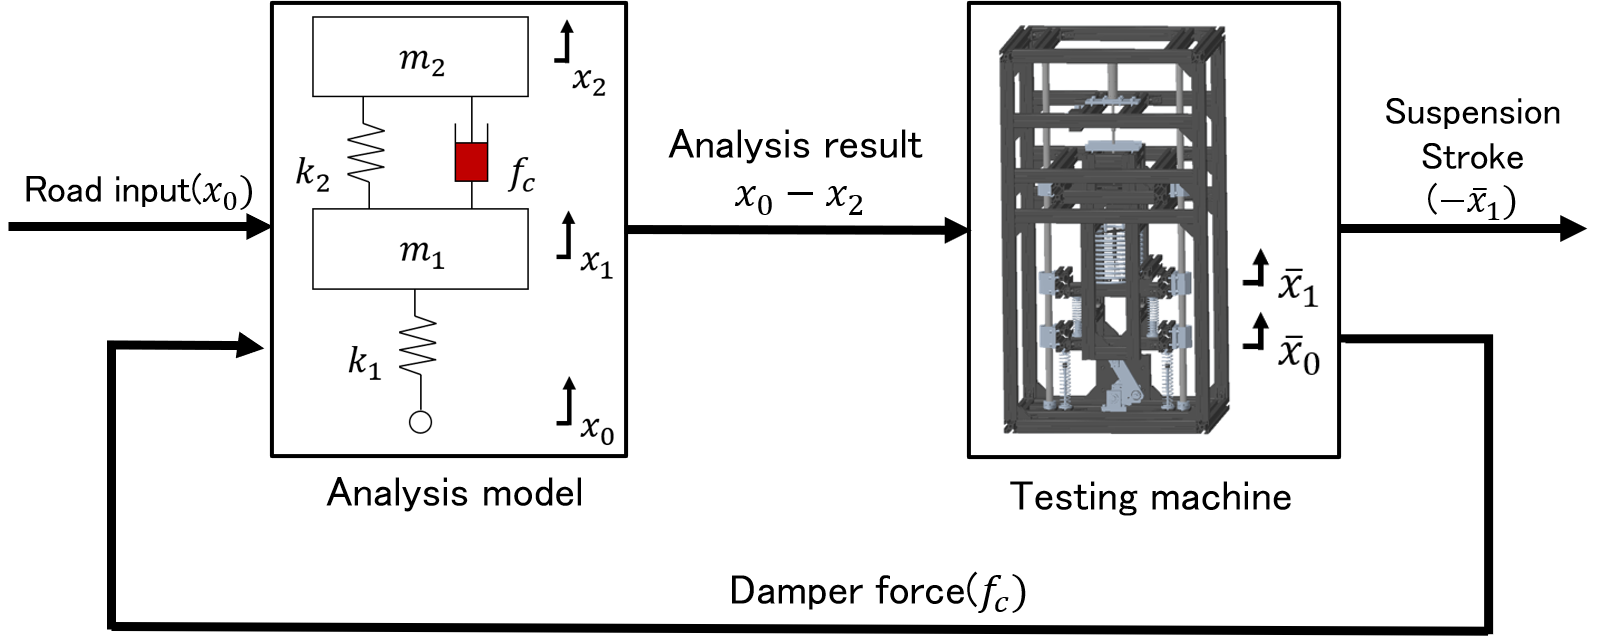
\includegraphics[height=40mm]{figure/relative_diagram.eps}
    \vspace*{3mm}
    \caption{Block diagram of HILS system(relative)}
    \label{fig:relative_diagram}
  \end{center}
\end{figure}

%------- IDCS --------------
\subsection{IDCSを用いた制御手法}
\label{sec:method_idcs}
\subsubsection{IDCS制御手法}
\label{sec:sub_method_idcs}
続いてIDCSを用いた制御手法について説明する.Inverse Dynamics Compensation via 'Simulation of feedback control system'(IDCS)制御手法はシステムの順動力学モデルを用いたフィードバック制御シミュレーションにより近似的な逆動力学の計算を行う手法である\cite{method_idcs}.図~\ref{fig:idcs_block}にIDCS制御手法のブロック線図を示す.点線で囲まれた部分は数値シミュレーション環境であり,$P_m$は制御対象$P$を模擬したモデルである.制御器$K$と$P_m$で構築されるフィードバック制御系はシミュレーション上では理想的な制御を行えるため,$P_m$の出力$y_m$は目標値$r$に追従する.ここで$P_m$と$P$が同一であると考えると,$P$の出力$y$は目標値$r$に追従する.IDCS制御手法は,制御対象からの物理フィードバックを必要としないため,センサレスな制御が可能となっている.

\vspace*{10mm}
\begin{figure}[htp]
  \begin{center}
    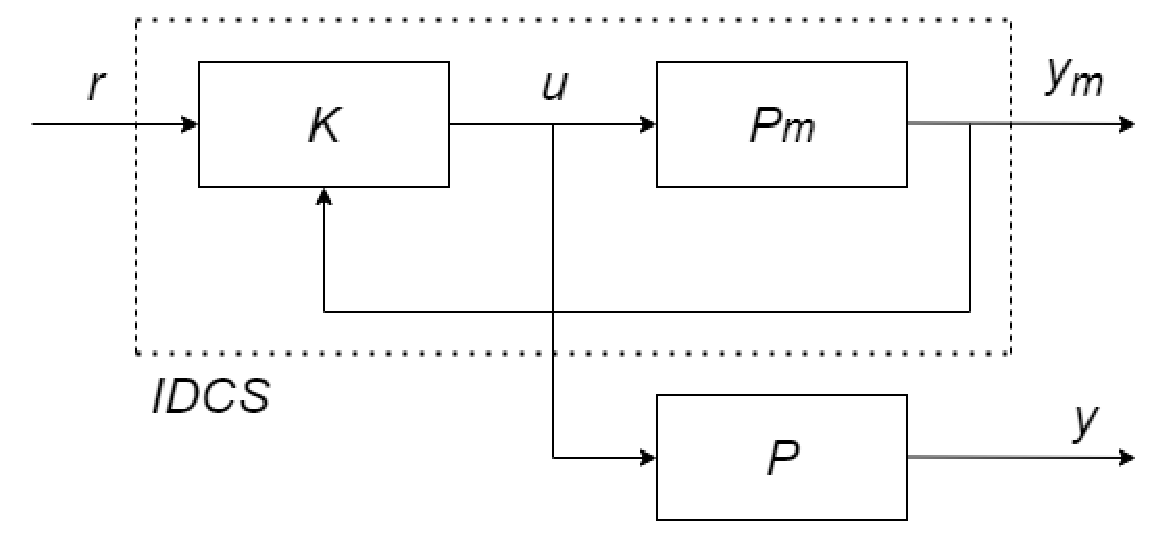
\includegraphics[height=40mm]{figure/idcs_block.eps}
    \vspace*{3mm}
    \caption{Block diagram(IDCS)}
    \label{fig:idcs_block}
  \end{center}
\end{figure}

\newpage

図~\ref{fig:idcs_block}~の点線で囲まれた部分は制御対象の逆動力学$P^{-1}$に対応している.図~\ref{fig:bode_inv_idcs}~に本研究の制御対象であるHILS試験機の逆伝達関数とIDCSの点線部の伝達関数のボード線図を示す.式(~\ref{eq:1dof}~)にIDCS制御系内の試験機を模擬したモデルの運動方程式,図~\ref{fig:hardware_model}~にHILS試験機のモデル図,表~\ref{tab:parameter_1dof}~にHILS試験機の諸元を示す,ボード線図から,IDCS制御系の制御器$K$の比例ゲインを大きくすることで,IDCS制御系の伝達関数はシステムの逆伝達関数に近づくことがわかる.

\begin{equation}
  m_1\ddot{\bar{x}}_1+c_2\dot{\bar{x}}_1+k_1(\bar{x}_1-\bar{x}_0)+k_2\bar{x}_1=0 \label{eq:1dof}
\end{equation}

ここで,$m_1$はタイヤ質量 ,$k_1$はタイヤの縦ばね剛性,$k_2$はばね定数,$c_2$は減衰係数,$\bar{x}_0$はHILS試験機の路面部変位,$\bar{x}_1$はタイヤ変位である.

\vspace{7mm}
\begin{figure}[htp]
  \begin{center}
    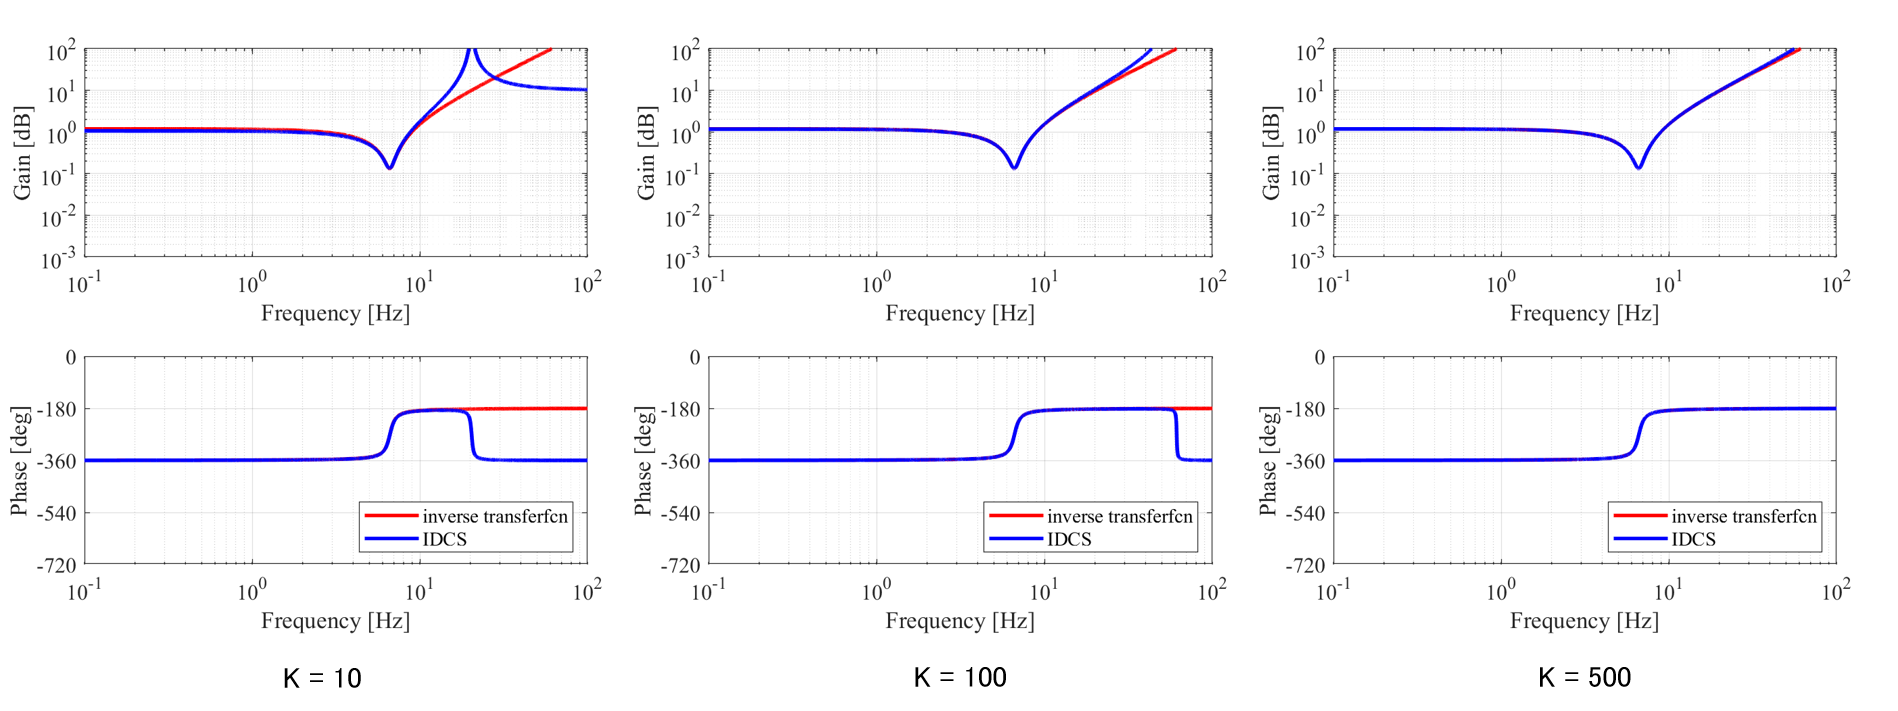
\includegraphics[height=65mm]{figure/bode_inverse.eps}
    \caption{Comparison of inverse transfer function and IDCS}
    \label{fig:bode_inv_idcs}
  \end{center}
\end{figure}
\vspace{7mm}
\begin{figure}[h]
  \begin{minipage}{0.4\hsize}
     \begin{center}
      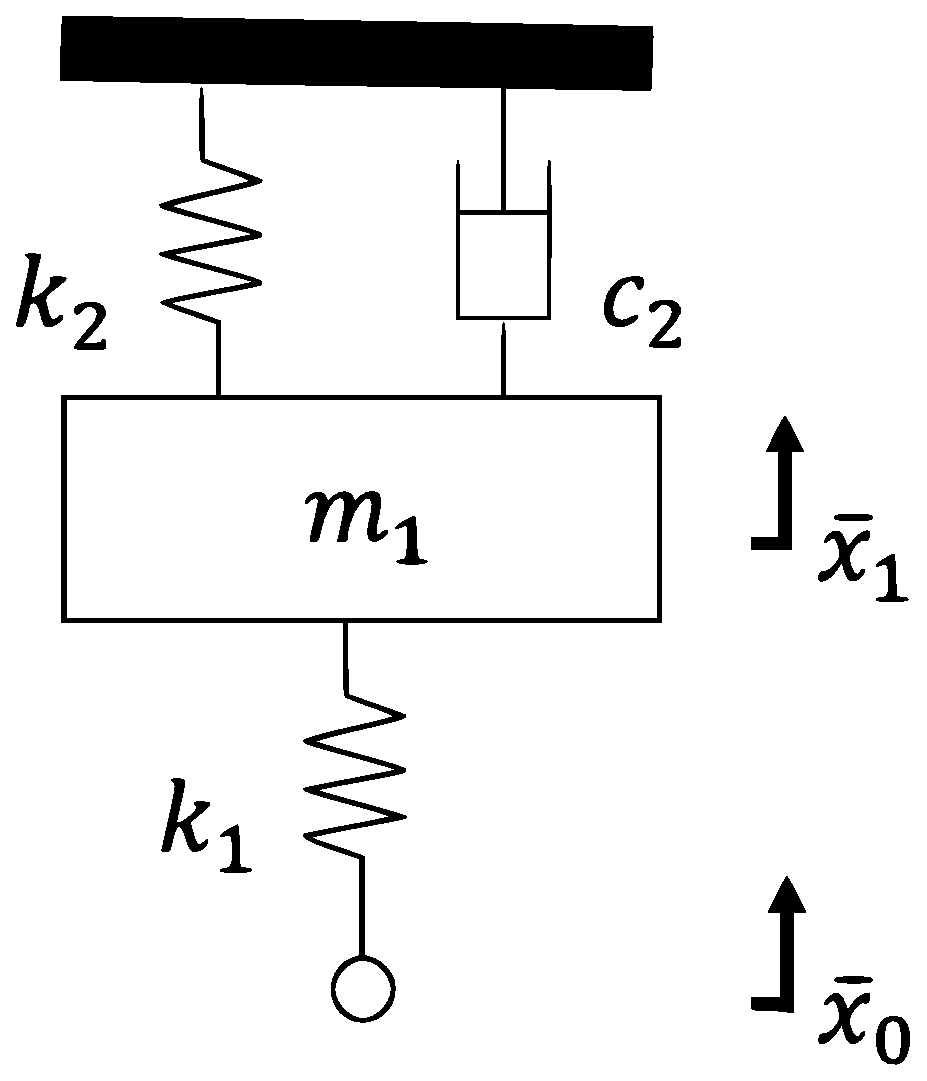
\includegraphics[height=45mm]{figure/hardware_model.eps}
	\vspace{2mm}
      \caption{Hardware Model}
      \label{fig:hardware_model}
    \end{center}
  \end{minipage}
  \vspace{7mm}
\begin{minipage}{0.6\hsize}
\makeatletter
\def\@captype{table}
\makeatother
  \begin{center}
   \caption{Parameter of 1DOF Model}
   \label{tab:parameter_1dof}
   \begin{tabular}{cc}\hline
      Unsprung Mass $m_1$ [kg] & 1.5  \\
      Vertical spring stiffness $k_1$ [N/m] & 2200  \\
      Spring constant $k_2$ [N/m] & 439   \\
      Damping coefficient $c_2$ [N/m] & 15   \\ \hline
    \end{tabular}
   \end{center}
 \end{minipage}
\end{figure}
\newpage

IDCS制御系を組み込んだHILSシステムのブロック線図を図~\ref{fig:idcs_diagram}~に示す.

\vspace*{7mm}
\begin{figure}[htp]
  \begin{center}
    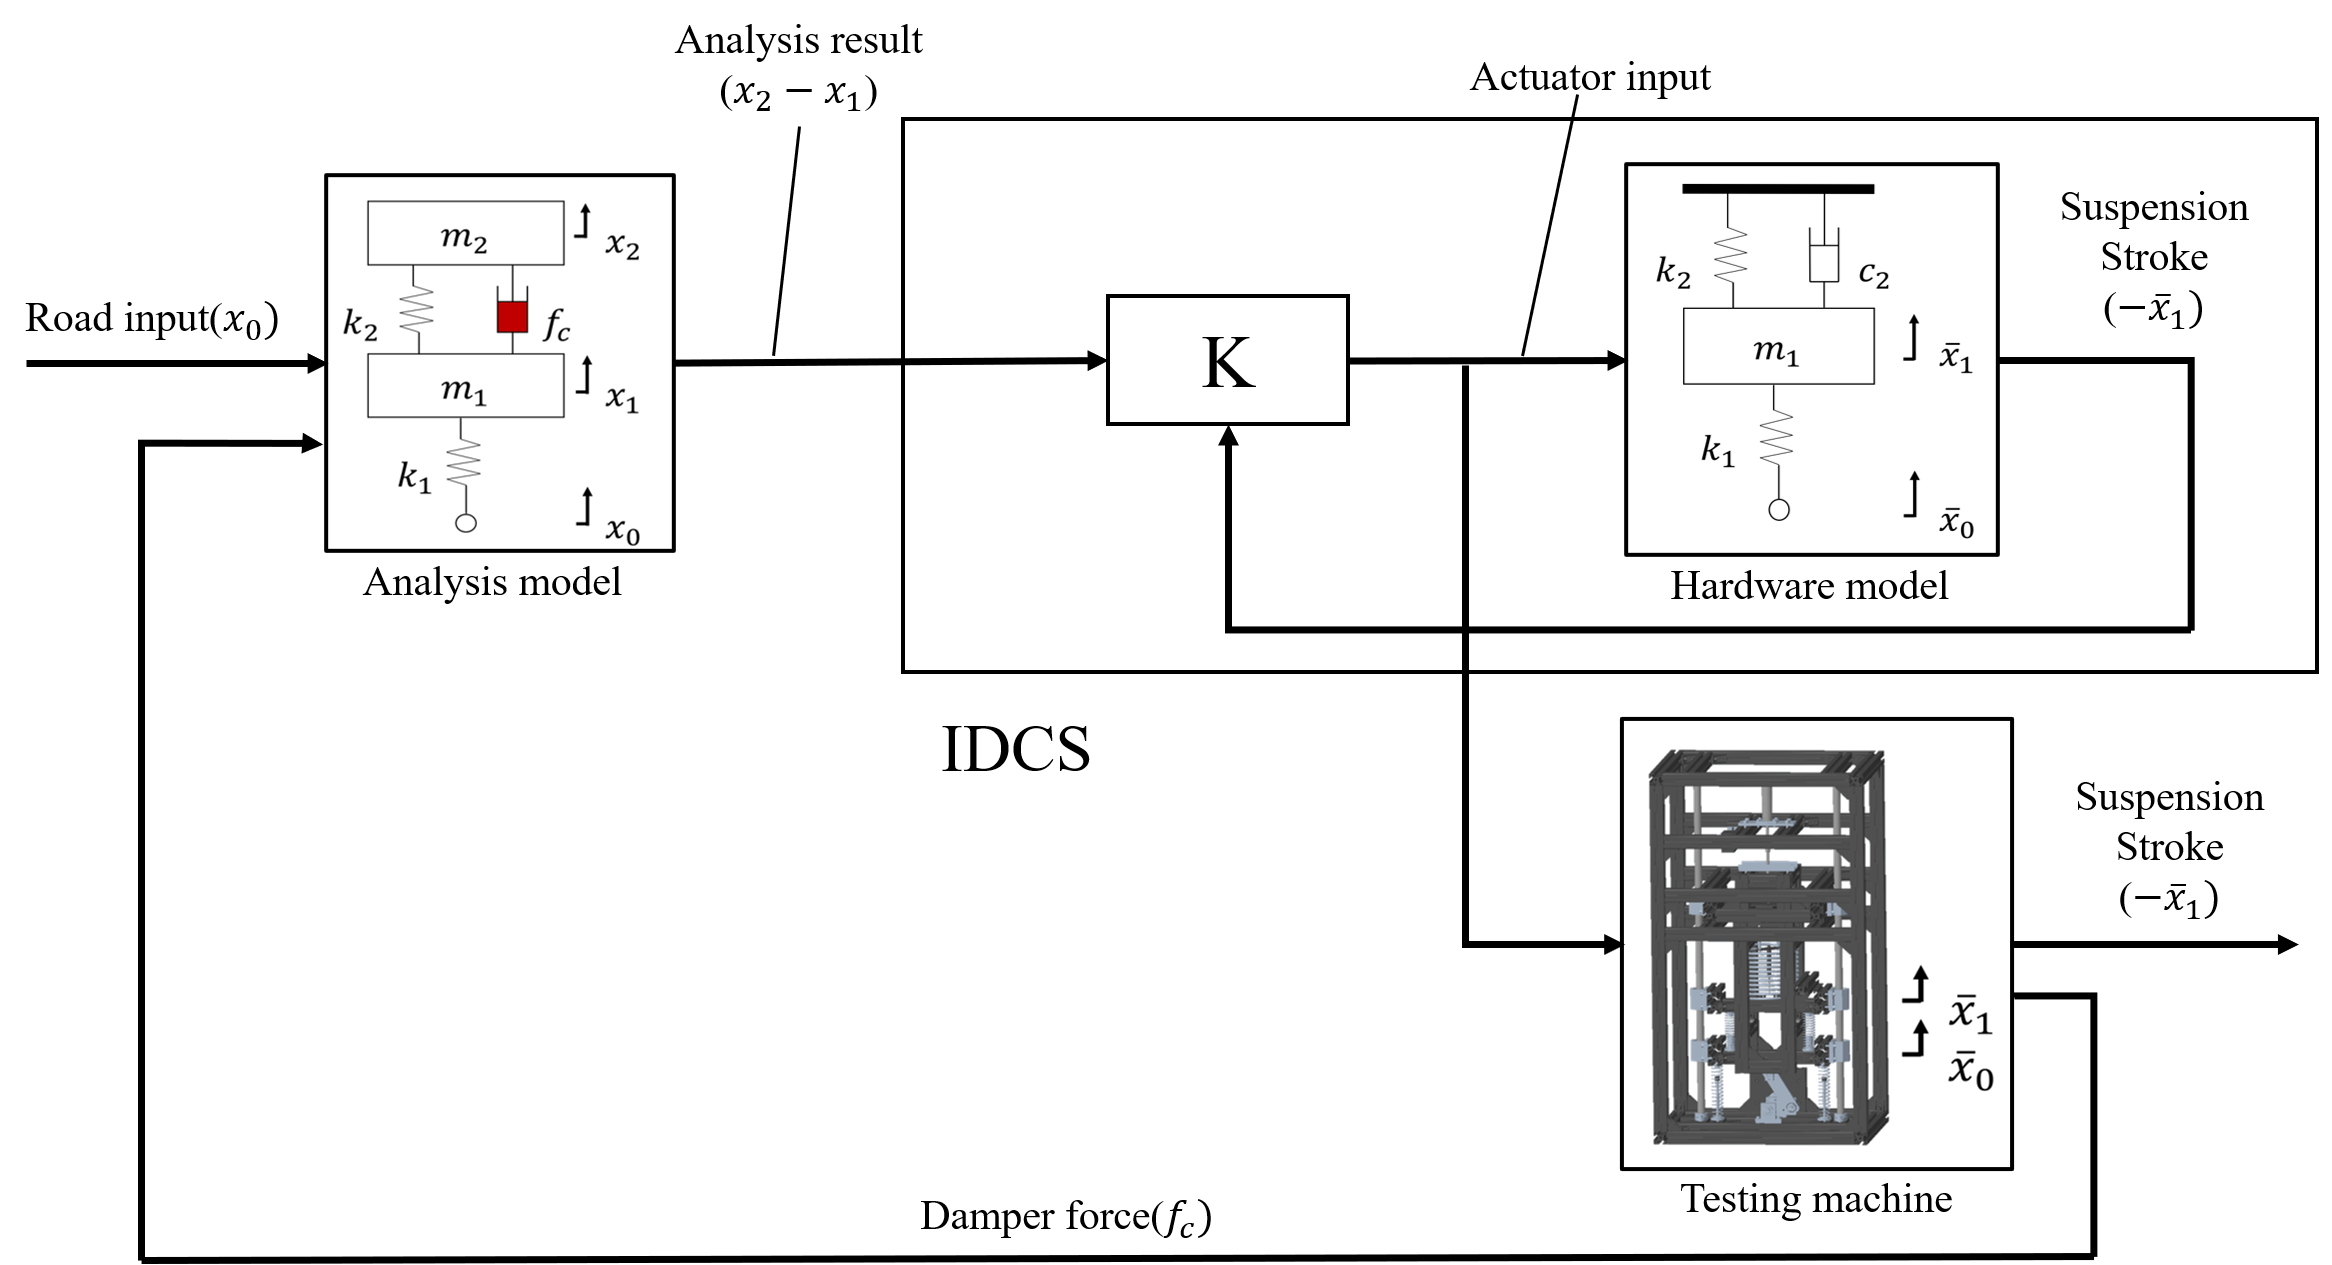
\includegraphics[height=90mm]{figure/idcs_diagram.eps}
    \vspace*{3mm}
    \caption{Block diagram of HILS system(IDCS)}
    \label{fig:idcs_diagram}
  \end{center}
\end{figure}
\newpage

\subsubsection{非線形ダンパモデル}
~\ref{sec:sub_method_idcs}章で述べた通り,IDCS制御手法において制御精度を高めるには,制御対象と制御対象モデルとのモデル化誤差を小さくする必要がある.そこで本研究で使用するダンパの単体試験を行い,試験データより作成した非線形性を考慮したダンパモデルを制御対象のモデルに組み込む..

シリンダ内の空気の密度と圧力をそれぞれ$\rho$,$P$,初期状態では,大気の密度$\rho_0$,大気圧$P_0$に等しいと仮定する.ダンパ力はシリンダ内の圧力変化$\Delta P = P-P_0$とダンパのピストン面積$S$より,式(~\ref{eq:delta_P})で表せる.

\begin{equation}
  F = \Delta PS \label{eq:delta_P}
\end{equation}

$\Delta P$は,式\ref{eq:q_m}の数値解を用いた.

空気の状態変化を断熱変化と仮定すると,式(~\ref{eq:insulation})で表せる.また,ピストン断面積を$S$とし,初期状態のシリンダ上端とピストン上面までの距離を$x_0$,ピストンの変位を$x$とする.空気の質量流量を$Q_m$とすると,質量保存則より式(~\ref{eq:conservation_mass})が成立する.

\begin{equation}
  \frac{P}{P_0} = \left(\frac{\rho}{\rho_0} \right)^\kappa \label{eq:insulation}
\end{equation}
\begin{equation}
  \rho_0 S x_0 = \rho S(x_0 - x) + \int Q_m dt \label{eq:conservation_mass}
\end{equation}

式(~\ref{eq:insulation}),式(~\ref{eq:conservation_mass})より微分方程式を導くと,式(~\ref{eq:damper_diff_eq})が表せる.

\begin{equation}
  \frac{1}{\kappa P_0} \frac{dP}{dt} \left(\frac{P}{P_0} \right)^{\frac{1}{\kappa} -1} \left(1 - \frac{x}{x_0} \right) - \left(\frac{P}{P_0} \right)^{\frac{1}{\kappa}} \frac{1}{x_0} \frac{dx}{dt} + \frac{1}{\rho_0 S x_0} Q_m = 0 \label{eq:damper_diff_eq}
\end{equation}

また,オリフィス流路内の空気の圧力,密度は近似的に$P_0$,$\rho_0$に等しいとし,オリフィス前後の流れに対して,ベルヌーイの式を適用するとその質量流量$Q_m$は式(~\ref{eq:q_m})と表せる.

\begin{equation}
  Q_m = sgn\left(P - P_0 \right)C_{or}S_{or}\sqrt{2 \rho \left(P-P_0 \right)} \label{eq:q_m}
\end{equation}

式(~\ref{eq:q_m})の流量係数$C_{or}$は実験的に求めるものである.

\newpage
作成した非線形ダンパモデルに正弦波入力を与え,振幅を変化させた時,周波数を変化させた時のF-X線図,F-V線図を図~\ref{fig:damper_x_3},図~\ref{fig:damper_3_x}に示す.

\vspace*{5mm}
\begin{figure}[h]
  \begin{tabular}{cc}
  \begin{minipage}{0.5\hsize}
  \begin{center}
    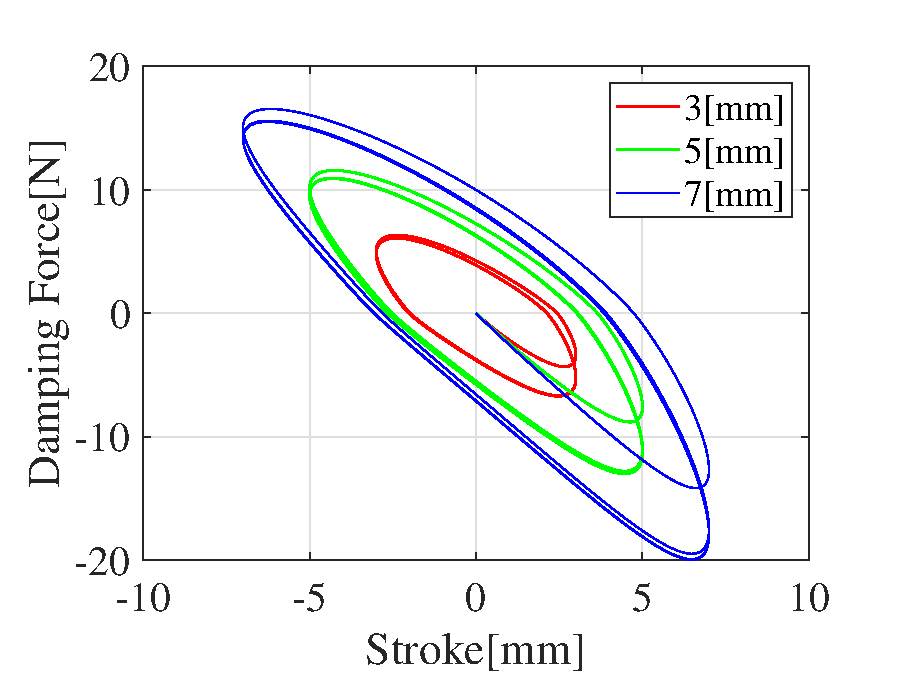
\includegraphics[height=40mm]{figure/damper_x_1_Fx.eps}
    \end{center}
    \begin{center}
    \ F-X\
    \end{center}
  \end{minipage}
  \begin{minipage}{0.5\hsize}
     \begin{center}
      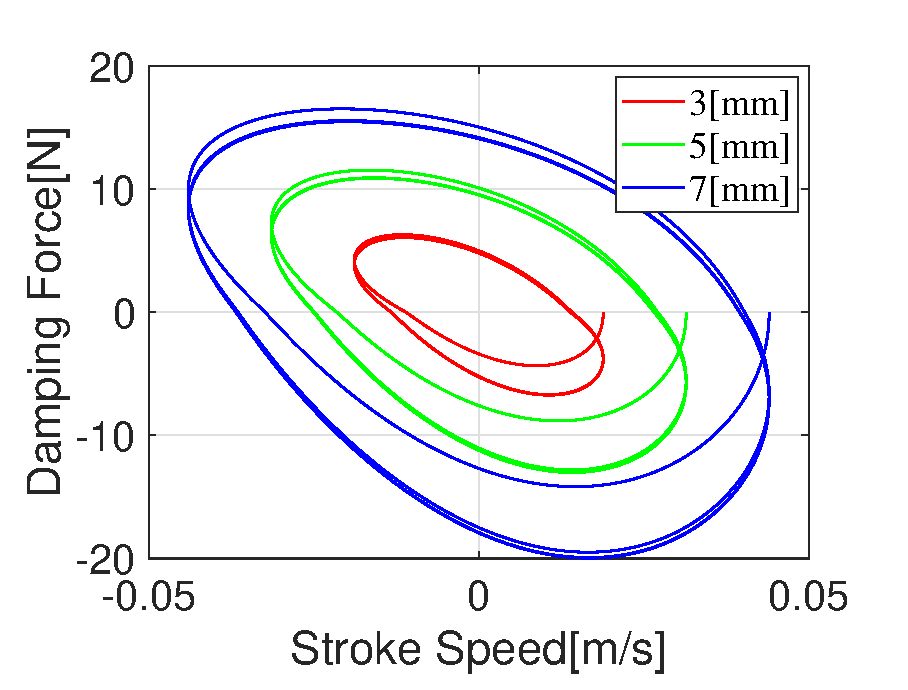
\includegraphics[height=40mm]{figure/damper_x_1_Fv.eps}
      \end{center}
      \begin{center}
      \ F-V\
    \end{center}
  \end{minipage}
  \end{tabular}
  \vspace*{3mm}
  \caption{Difference in amplitude(Frequency:1Hz)}
    \label{fig:damper_x_3}
\end{figure}

\vspace*{10mm}
\begin{figure}[h]
  \begin{tabular}{cc}
  \begin{minipage}{0.5\hsize}
  \begin{center}
    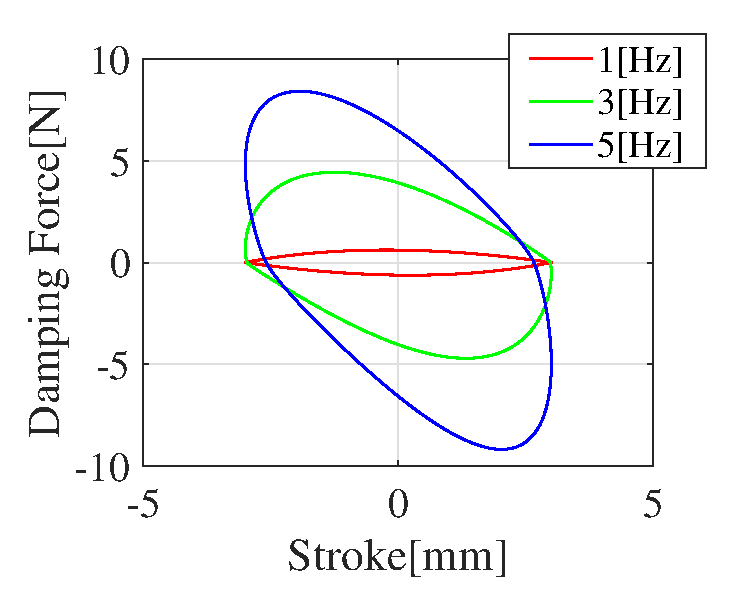
\includegraphics[height=40mm]{figure/damper_3_x_Fx.eps}
    \end{center}
    \begin{center}
    \ F-X\
    \end{center}
  \end{minipage}
  \begin{minipage}{0.5\hsize}
     \begin{center}
      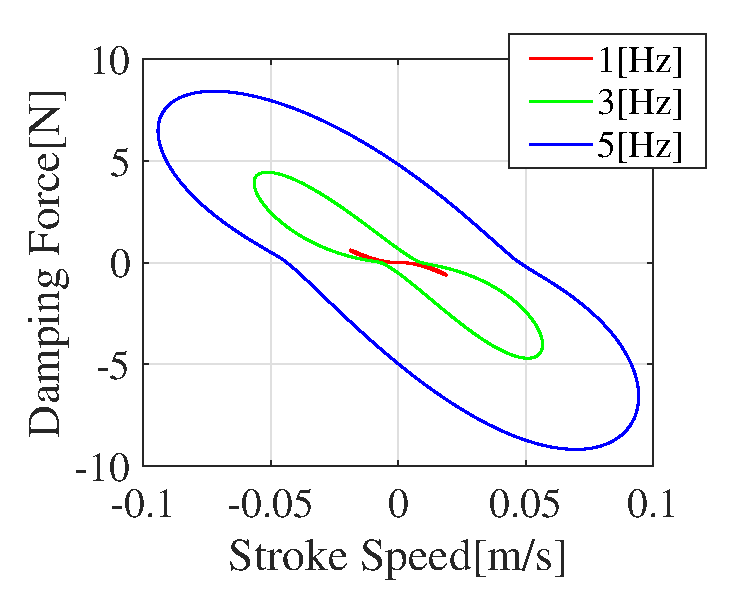
\includegraphics[height=40mm]{figure/damper_3_x_Fv.eps}
      \end{center}
      \begin{center}
      \ F-V\
    \end{center}
  \end{minipage}
  \end{tabular}
  \vspace*{3mm}
  \caption{Difference in frequency(Amplitude:3mm}
    \label{fig:damper_3_x}
\end{figure}
\newpage

\section{制御手法によるHILSシステムの評価}
\subsection{シミュレーションによる評価}
HILSシステムを用いて試験をする前にハードウェア部を1自由度モデルに置き換え,シミュレーションを行った.シミュレーション時の相対変位による制御手法のブロック線図を図~\ref{fig:sim_block_relative}~に,IDCS制御手法のブロック線図を図~\ref{fig:sim_block_idcs}~に示す.解析モデルで計算したサスペンションストロークとハードウェアのモデルで計算されたサスペンションストロークを比較し,各制御手法の評価を行う.今回,HILS試験機のサスペンションストロークの範囲が25mmであるため,その範囲を超えない上でシミュレーションを行った.ハードウェアのモデルは~\ref{sec:method_idcs}~節で述べたモデルを用いる.

\vspace*{5mm}
\begin{figure}[htp]
  \begin{center}
    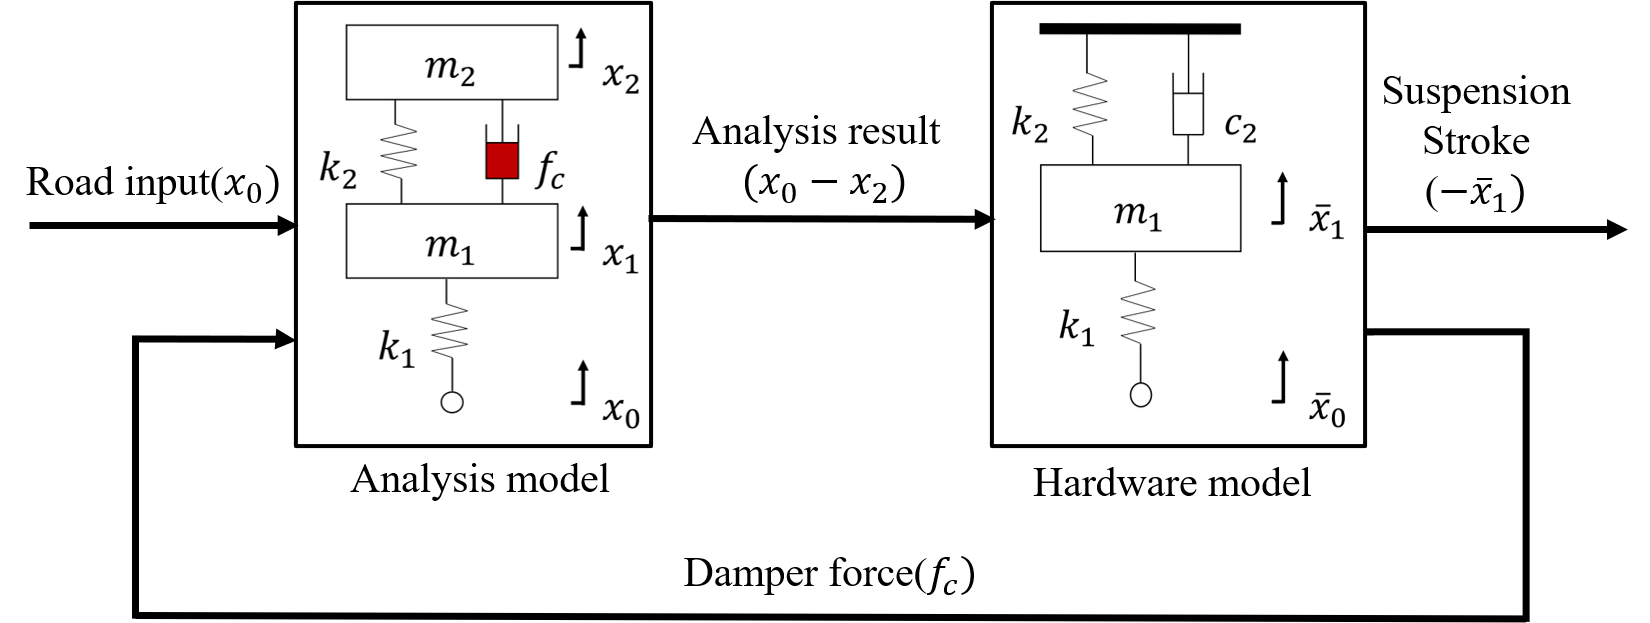
\includegraphics[height=45mm]{figure/sim_block_diagram(relative).eps}
    \vspace*{3mm}
    \caption{Block diagram in simulation(Relative)}
    \label{fig:sim_block_relative}
  \end{center}
\end{figure}

\begin{figure}[htp]
  \begin{center}
    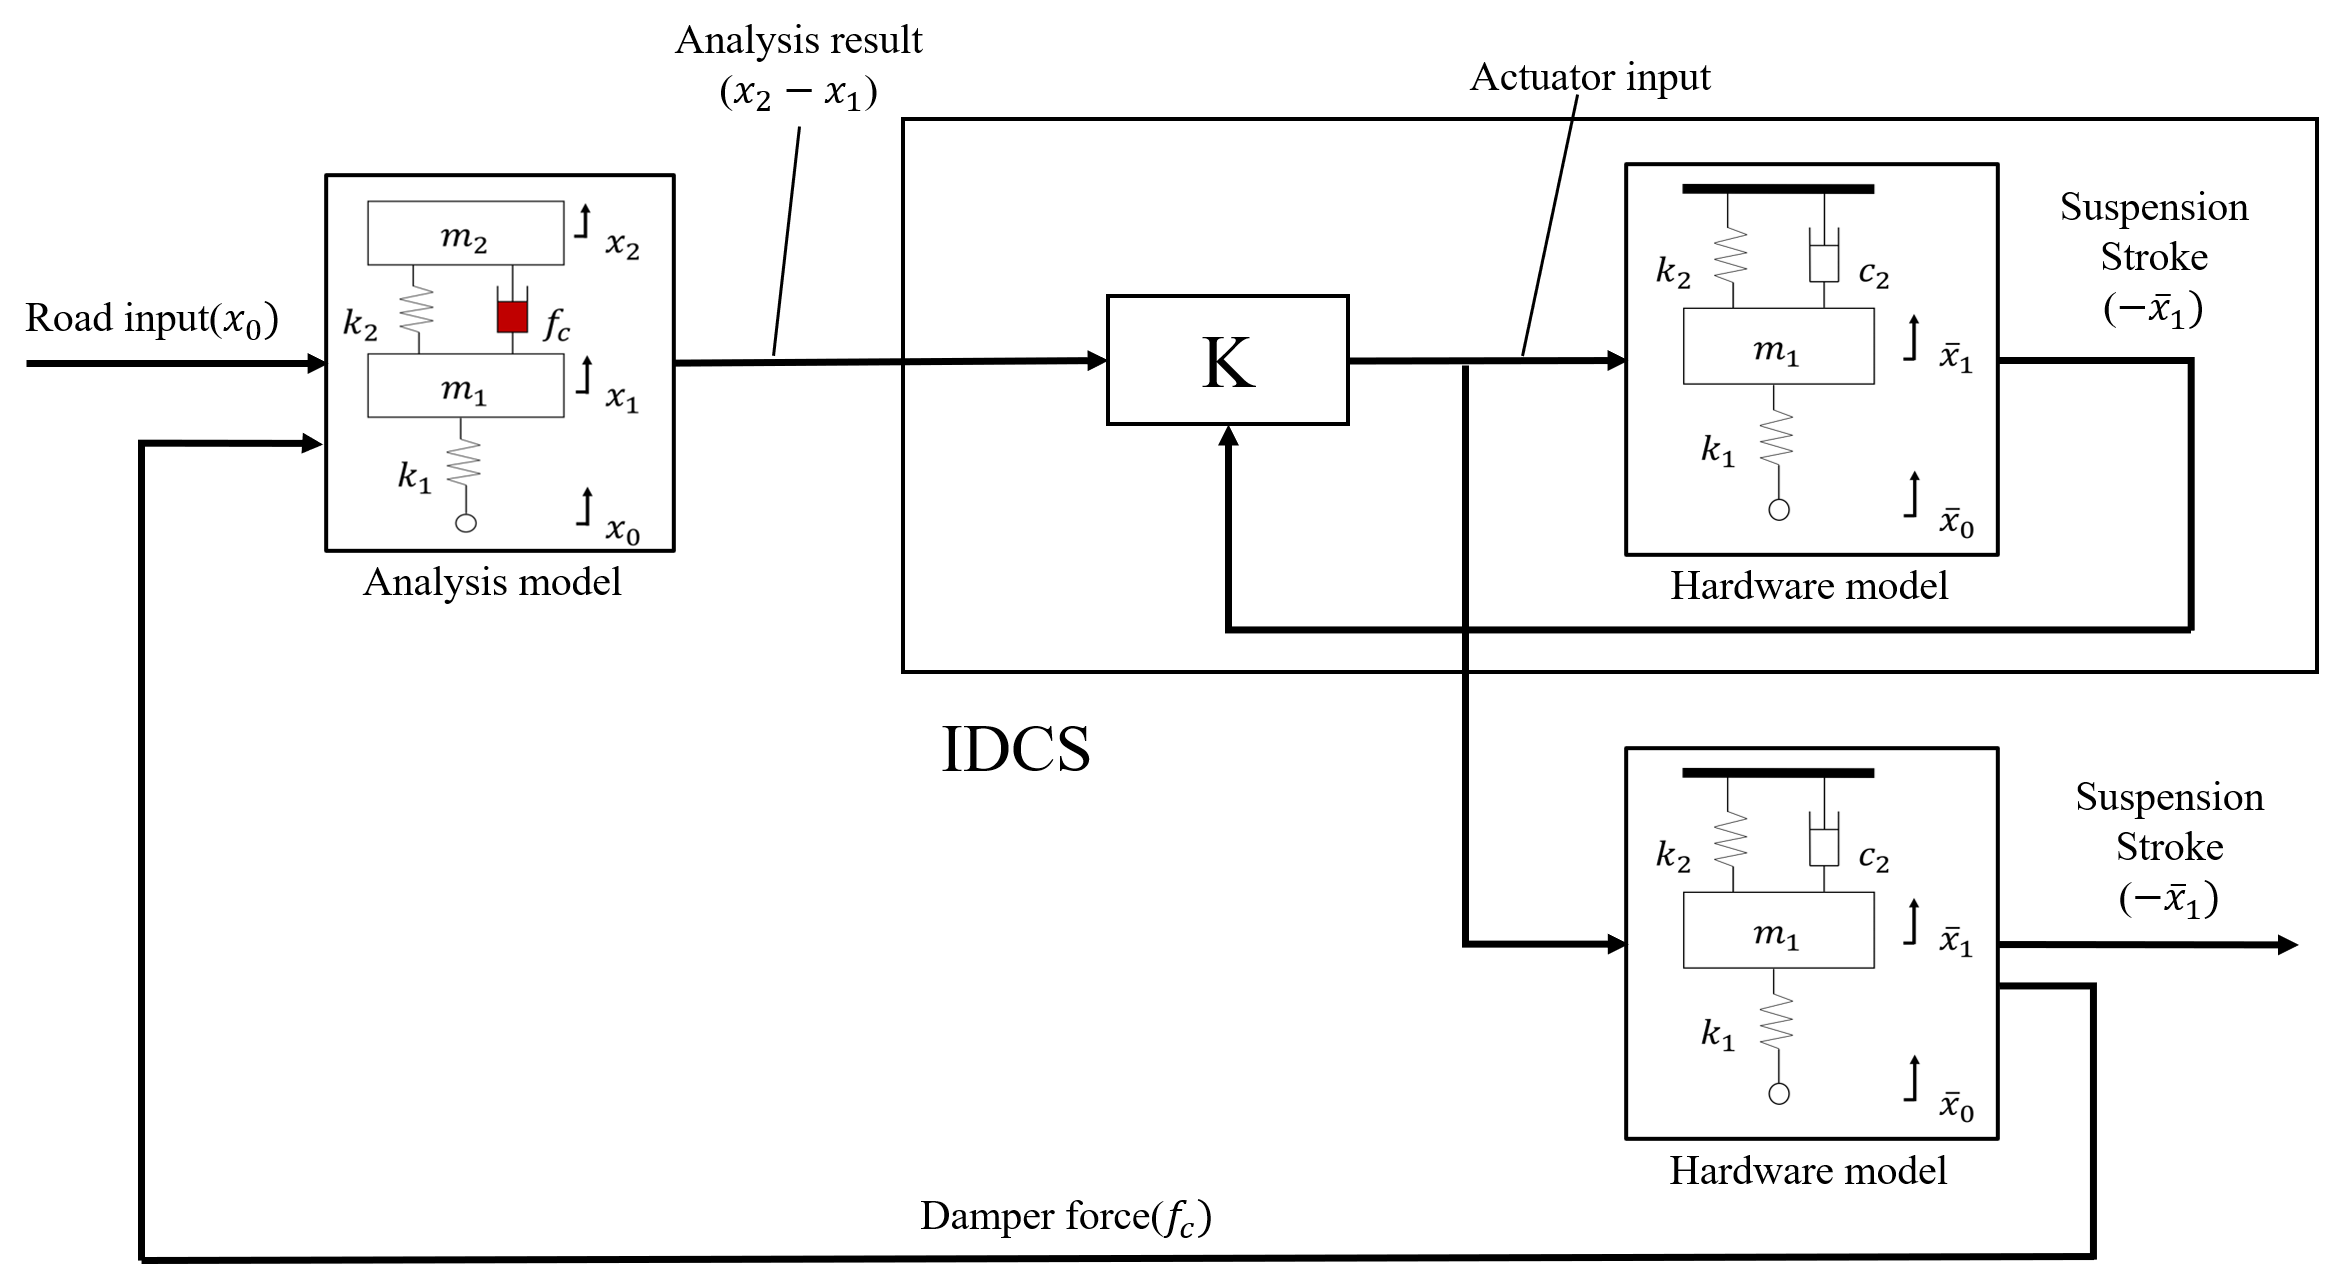
\includegraphics[height=85mm]{figure/sim_block_diagram(idcs).eps}
    \vspace*{3mm}
    \caption{Block diagram in simulation(IDCS)}
    \label{fig:sim_block_idcs}
  \end{center}
\end{figure}

\newpage
図~\ref{fig:sim_5_1}に周波数1.0Hz,振幅5mmの正弦波入力,図~\ref{fig:sim_3_3}に周波数3.0Hz,振幅3mm,図~\ref{fig:sim_5_1}に周波数5.0Hz,振幅2mmの正弦波を路面入力としたときのサスペンションストロークを,各手法ごとに比較したグラフを示す.解析モデルで計算したサスペンションストロークとハードウェアのモデルで計算した結果を示す.

シミュレーション結果より,IDCSを用いた制御手法では,制御器$K$の比例ゲイン$K_p$を大きくするほど,ハードウェアのモデルの計算結果は,解析モデルで計算したサスペンションストロークに近づくことがわかる.また相対変位による制御手法は,周波数を大きくするとハードウェアの計算結果は,解析モデルで計算したサスペンションストロークから離れるが,IDCSによる制御手法では周波数を大きくしてもハードウェアの計算結果が,解析モデルのサスペンションストロークに近いことがわかる.

\vspace*{5mm}
\begin{figure}[h]
  \begin{tabular}{cc}
  \begin{minipage}{0.5\hsize}
  \begin{center}
    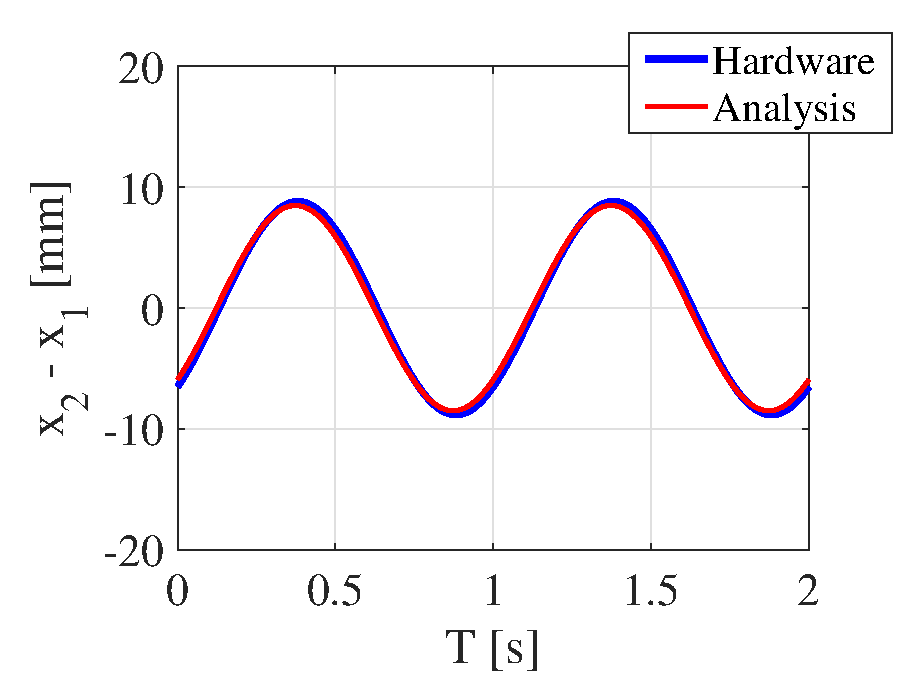
\includegraphics[height=35mm]{figure/sim_rela_5_1.eps}
    \end{center}
    \begin{center}
    \ (a)Relative\
    \end{center}
  \end{minipage}
  \begin{minipage}{0.5\hsize}
     \begin{center}
      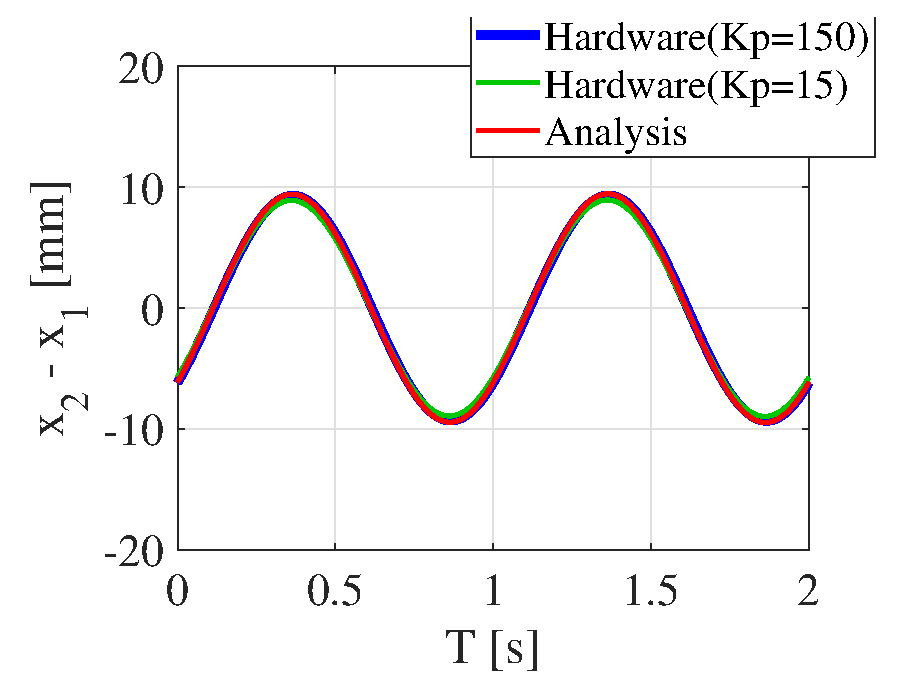
\includegraphics[height=35mm]{figure/sim_idcs_5_1.eps}
      \end{center}
      \begin{center}
      \ (b)IDCS\
    \end{center}
  \end{minipage}
  \end{tabular}
  \vspace*{2mm}
  \caption{Comparison of Suspension Stroke(Input:1Hz 5mm)}
    \label{fig:sim_5_1}
\end{figure}
\begin{figure}[h]
  \begin{tabular}{cc}
  \begin{minipage}{0.5\hsize}
  \begin{center}
    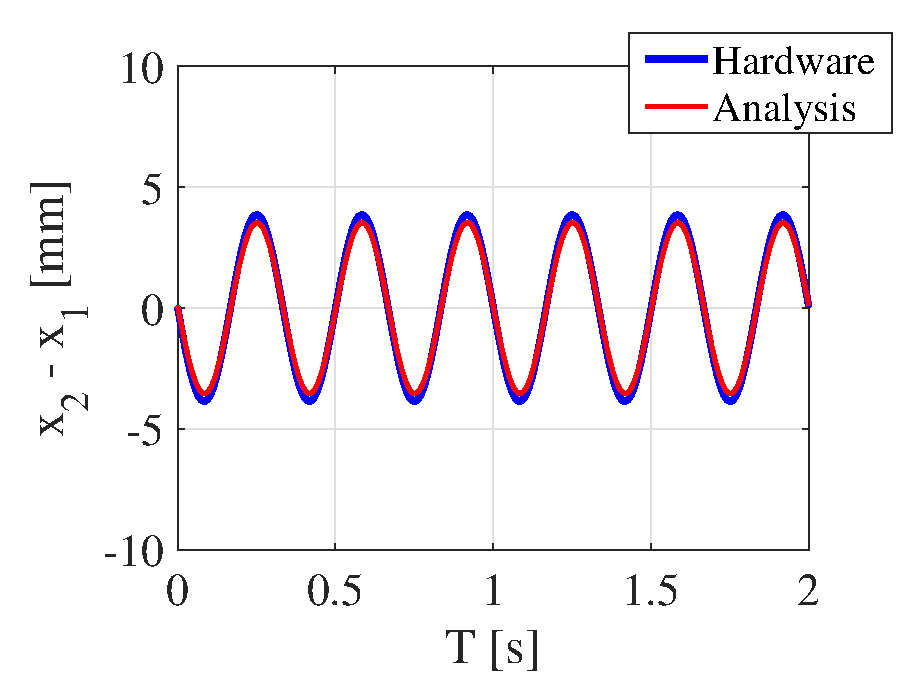
\includegraphics[height=35mm]{figure/sim_rela_3_3.eps}
    \end{center}
    \begin{center}
    \ (a)Relative\
    \end{center}
  \end{minipage}
  \begin{minipage}{0.5\hsize}
     \begin{center}
      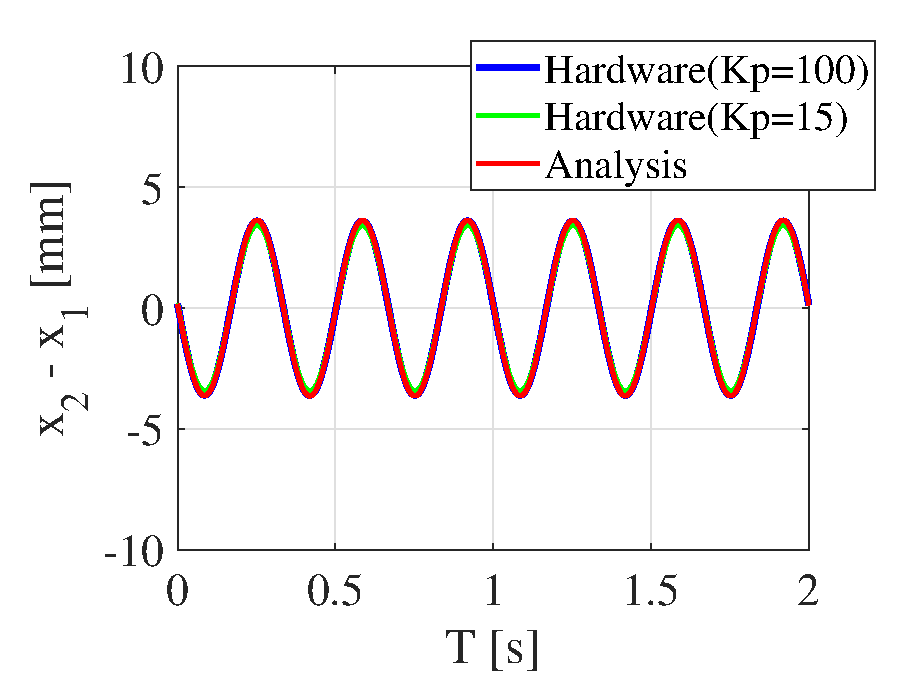
\includegraphics[height=35mm]{figure/sim_idcs_3_3.eps}
      \end{center}
      \begin{center}
      \ (b)IDCS\
    \end{center}
  \end{minipage}
  \end{tabular}
  \vspace*{2mm}
  \caption{Comparison of Suspension Stroke(Input:3Hz 3mm)}
  \label{fig:sim_3_3}
\end{figure}
\begin{figure}[h]
  \begin{tabular}{cc}
  \begin{minipage}{0.5\hsize}
  \begin{center}
    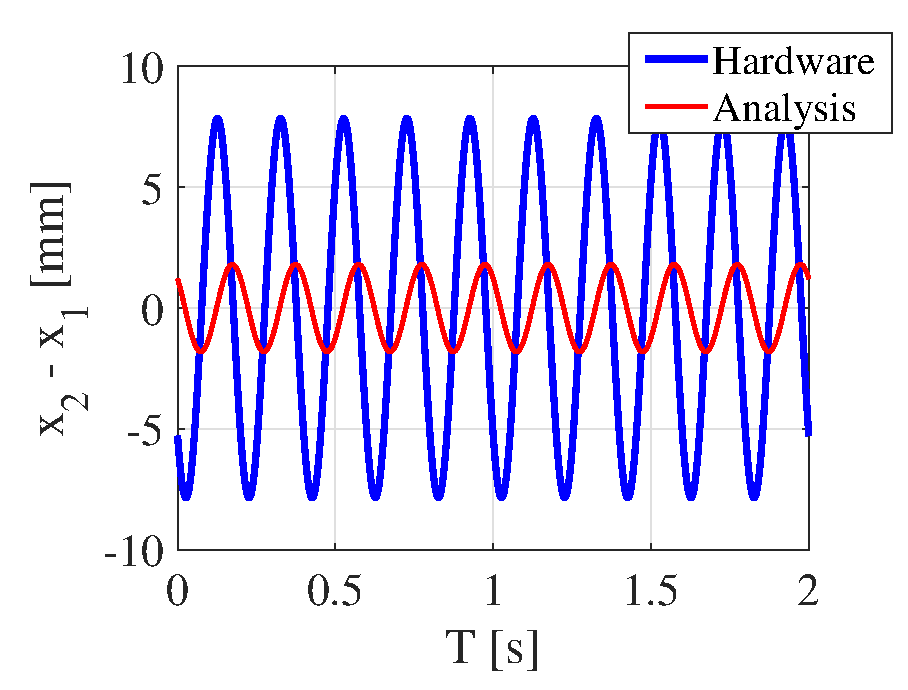
\includegraphics[height=35mm]{figure/sim_rela_2_5.eps}
    \end{center}
    \begin{center}
    \ (a)Relative\
    \end{center}
  \end{minipage}
  \begin{minipage}{0.5\hsize}
     \begin{center}
      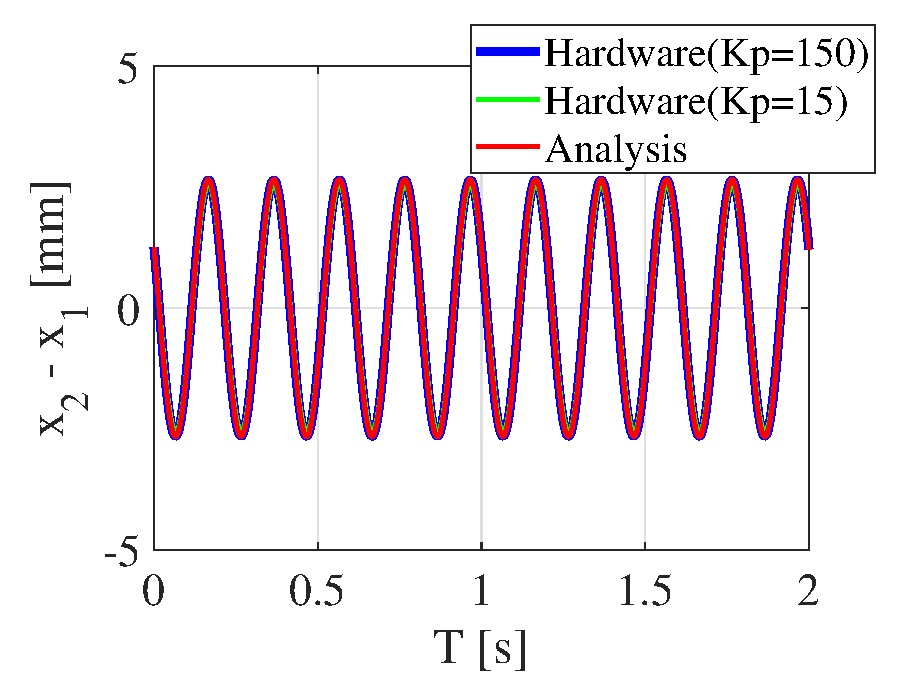
\includegraphics[height=35mm]{figure/sim_idcs_2_5.eps}
      \end{center}
      \begin{center}
      \ (b)IDCS\
    \end{center}
  \end{minipage}
  \end{tabular}
  \vspace*{2mm}
  \caption{Comparison of Suspension Stroke(Input:5Hz 2mm)}
  \label{fig:sim_2_5}
\end{figure}

\newpage
非線形ダンパモデルを組み込んだIDCS制御手法による制御手法のシミュレーション結果を図~\ref{}に示す.

\newpage
\subsection{HILS試験}
検討した相対変位による制御手法とIDCSを用いた制御手法におけるHILSシステムの再現性を評価するために路面入力試験を行った.図~\ref{fig:hils_5_1}に周波数1.0Hz,振幅5mm,図~\ref{fig:hils_3_3}に周波数3.0Hz, 振幅3mmの正弦波を路面に入力した時の,解析モデルと試験機のサスペンションストロークを比較したグラフを示す.

\vspace{5mm}
\begin{figure}[h]
  \begin{tabular}{cc}
  \begin{minipage}{0.5\hsize}
  \begin{center}
    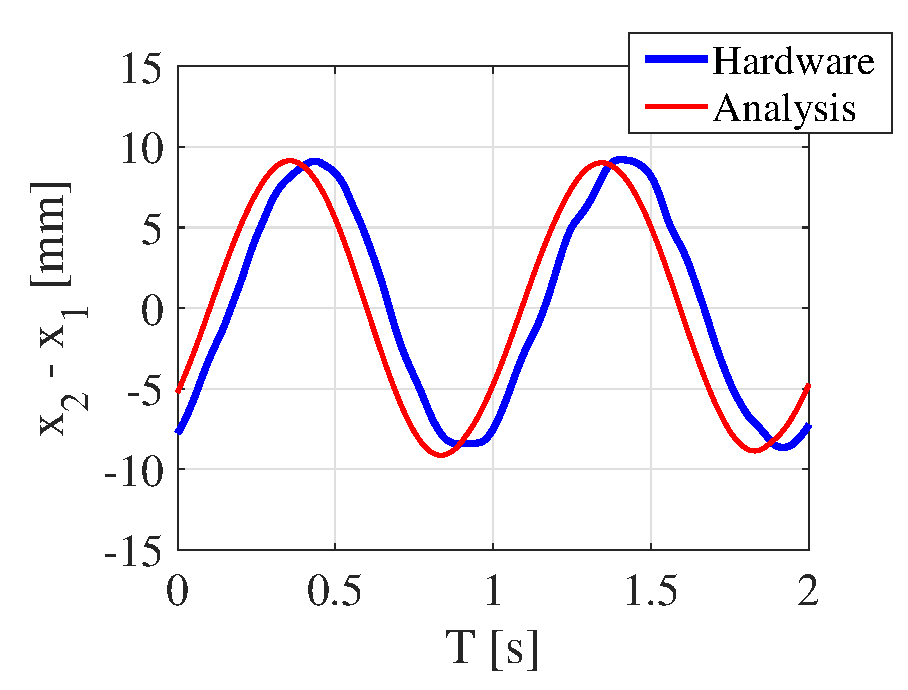
\includegraphics[height=40mm]{figure/hils_rela_5_1.eps}
    \end{center}
    \begin{center}
    \ (a)Relative\
    \end{center}
  \end{minipage}
  \begin{minipage}{0.5\hsize}
     \begin{center}
      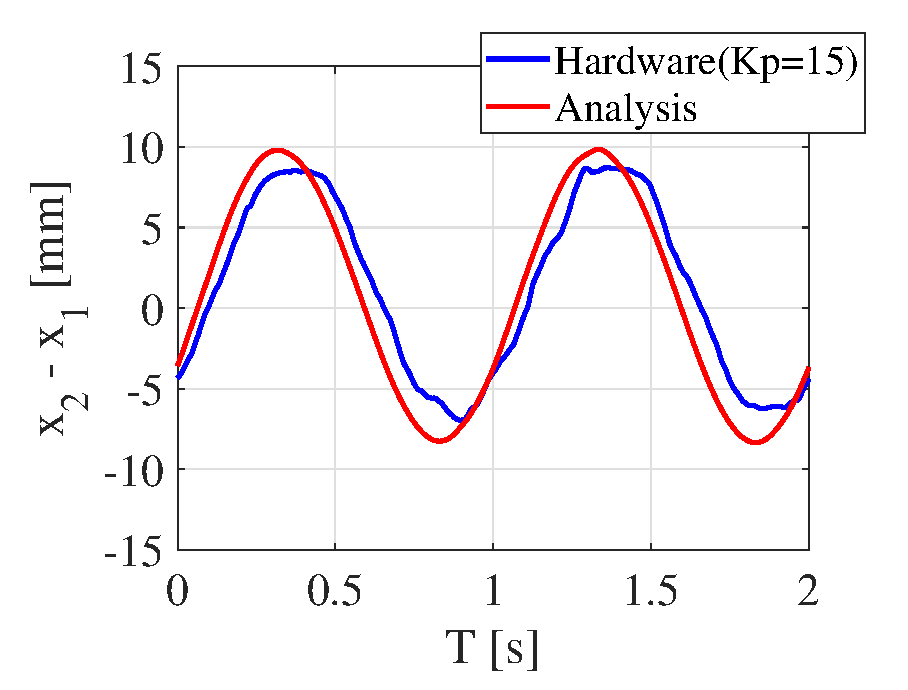
\includegraphics[height=40mm]{figure/hils_idcs_5_1.eps}
      \end{center}
      \begin{center}
      \ (b)IDCS\
    \end{center}
  \end{minipage}
  \end{tabular}
  \vspace*{2mm}
  \caption{Comparison of Suspension Stroke(Input:1Hz 5mm)}
    \label{fig:hils_5_1}
\end{figure}
\begin{figure}[h]
  \begin{tabular}{cc}
  \begin{minipage}{0.5\hsize}
  \begin{center}
    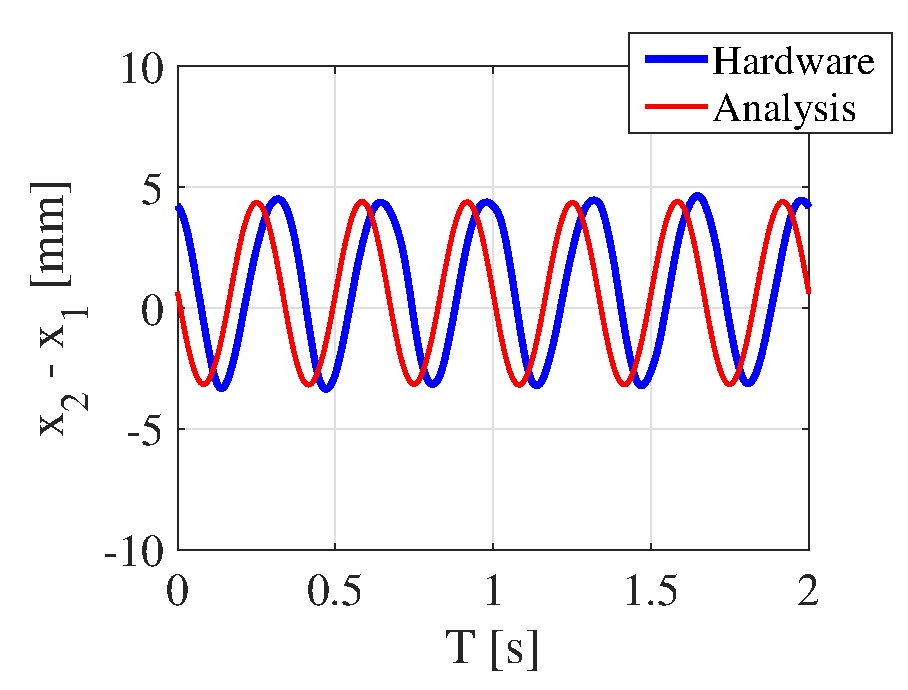
\includegraphics[height=40mm]{figure/hils_rela_3_3.eps}
    \end{center}
    \begin{center}
    \ (a)Relative\
    \end{center}
  \end{minipage}
  \begin{minipage}{0.5\hsize}
     \begin{center}
      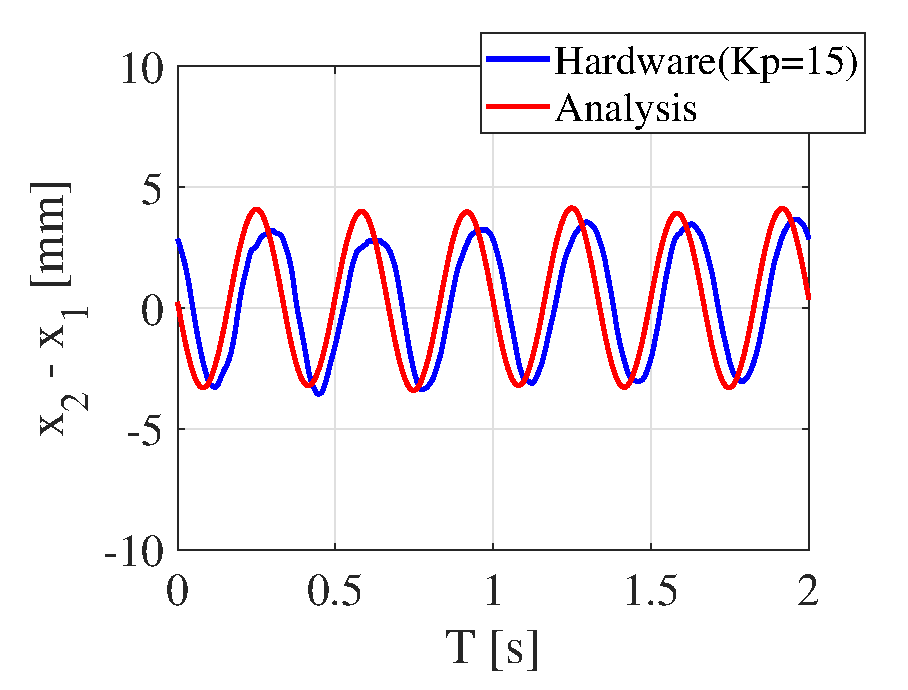
\includegraphics[height=40mm]{figure/hils_idcs_3_3.eps}
      \end{center}
      \begin{center}
      \ (b)IDCS\
    \end{center}
  \end{minipage}
  \end{tabular}
  \vspace*{2mm}
  \caption{Comparison of Suspension Stroke(Input:3Hz 3mm)}
    \label{fig:hils_3_3}
\end{figure}

\newpage
\section{結論}



% ----------シミュレーション結果を載せるよ~ ---------------------


\newpage
\begin{thebibliography}{99}
\bibitem{uno}宇野高明,車両運動性能とシャシーメカニズム,グランプリ出版,1994
\bibitem{nasugawa}茄子川捷久,宮下義孝,汐川満則,自動車の走行性能と試験方法,山海堂,2004
\bibitem{pic_sus.net}https://nge.jp/wp-content/uploads/2015/08/shutterstock\_22066612.jpg
\bibitem{exp_hils1}永井正夫,吉田秀久,Noomwongs Nuksit,横井隆,川眞田智,小林克宏,タイヤHIL シミュレータによる車両運動性能の研究(第1報) : タイヤHIL シミュレータの開発,自動車技術会論文集,Vol35,No.2,(2004),pp.147-152
\bibitem{exp_hils2}山口輝也, 実ヨーダンパを用いたHardware-In-the-Loopシミュレーションによる鉄道車両の蛇行動安定性試験(試験環境の構築と安定的な検証), 日本機械学会論文集,C編Vol.79 No.806(2013-10),pp.131-142
\bibitem{toyota_hils}https://www.toyota.co.jp/jpn/company/history/75years/data/automotive\_business/ \\ products\_technology/technology\_development/performance/images/supplement\_img01.jpg
\bibitem{dspace}http://www.dspace.com/ja/jpn/home.cfm
\bibitem{carbody_model}社団法人\ 自動車技術会,自動車技術ハンドブック5設計(シャシ)編,社団法人\ 自動車技術会,(1990),p. 25
\bibitem{method_idcs}青木 健悟,IDCSを用いた柔軟アームを有するロボットの振動制御,日本ロボット学会誌,Vol.31,No.10,(2010),pp.1001-1008

\bibitem{maxon}$\rm{http://academy.maxonjapan.co.jp/mmc}$

\end{thebibliography}

\end{document}
